\documentclass[12pt]{article}

\usepackage{setspace}         % Package for line spacing control
\usepackage{blindtext}        % For sample text (optional, remove for your real document)

% Commands for double spacing
\doublespacing % Applies double spacing to the main body, not footnotes/tables [2, 7, 8].

% OR use \linespread for a more direct factor (e.g., 2.0 for double) [8, 10].
% \linespread{2.0}

\usepackage{amsmath}
\usepackage{graphicx}
\usepackage{natbib}
\usepackage{hyperref}
\usepackage{amssymb,amsfonts}
\usepackage{booktabs}
\usepackage{multirow}
\usepackage{array}
\usepackage{utfsym}

\usepackage{times}
\usepackage[cm]{fullpage}
\usepackage{fancyhdr}
\usepackage{enumitem}
\usepackage{pdfpages}

\setlength{\headheight}{30pt}
\setlength{\headsep}{10pt}
\usepackage[top=3cm, bottom=1in, left=0.97in, right=0.97in]{geometry}
\pagestyle{fancyplain}
% \pagenumbering{gobble}
\lhead{\textbf{{Tung Lam Nguyen}  \\ \small\texttt{nguyenlamtung10@gmail.com} }}
\chead{{\LARGE \bf Dissertation} }
\rhead{
\includegraphics[height=0.85cm]{logo}}

\DeclareMathOperator*{\argmin}{argmin}

% \title{Penalty learning for Optimal Partitioning via Interval Regression}
% \author{Tung Lam Nguyen}
\date{}

\begin{document}

\begin{titlepage}
\thispagestyle{empty}

\begin{center}

% TITLE (ALL CAPS)
{\MakeUppercase{PENALTY LEARNING FOR OPTIMAL PARTITIONING VIA INTERVAL REGRESSION}}\\
\vspace{2\baselineskip}

% By line (double-spaced, no colon)
By\\
\vspace{\baselineskip}
\MakeUppercase{Tung L Nguyen}\\

\vspace{2\baselineskip}

A Dissertation\\
Submitted in Partial Fulfillment\\
of the Requirements for the Degree of\\
Doctor of Philosophy\\
in Informatics and Computing\\

\vspace{2\baselineskip}

Northern Arizona University\\
May 2026\\

\vfill

Approved:\\
\vspace{\baselineskip}

Jarrett Jay Barber, Ph.D., Chair\\
Toby Dylan Hocking, Ph.D., Co-chair (advisor)\\
Lan Zhang, Ph.D.\\
Alex Groce, Ph.D.\\

\end{center}

\end{titlepage}

% %----------------------------------------
% % Abstract
% %----------------------------------------
\clearpage
\setcounter{page}{2}
\renewcommand{\thepage}{\roman{page}}

\phantomsection
\addcontentsline{toc}{section}{ABSTRACT}

\thispagestyle{empty}

\begin{center}
ABSTRACT\\
\MakeUppercase{PENALTY LEARNING FOR OPTIMAL PARTITIONING VIA INTERVAL REGRESSION}\\
\MakeUppercase{Tung L Nguyen}
\end{center}

Changepoint detection identifies points in a sequence where the underlying data distribution changes, and it is widely used in fields such as finance, genomics, and healthcare. Dynamic programming algorithms, particularly those in the Optimal Partitioning (OP) family, are commonly used to detect changepoints efficiently. These methods rely on a penalty parameter to control the number of detected changepoints, but choosing an appropriate penalty is challenging: too low a penalty can lead to over-segmentation, while too high a penalty can miss important changes.
Traditionally, penalty selection has been based on manually computed features of the sequence and simple predictive models, such as linear or tree-based regression. However, these approaches often fail to capture the complex, non-linear relationship between sequence characteristics and the optimal penalty. Furthermore, the optimal penalty is not a single value but lies within a range, which naturally motivates modeling the problem as interval regression.
This thesis explores interval regression as a framework for learning penalty values in changepoint detection. I review existing interval regression methods and compare their performance on both synthetic and real-world datasets. Building on this, I propose learning-based approaches for predicting penalties directly from data, including multilayer perceptrons (MLPs) for continuous prediction and recurrent neural networks (RNNs) for sequences with temporal dependencies. These models reduce the need for manual feature engineering and better capture non-linear patterns in the data.
Experiments on benchmark genomic datasets show that interval regression–based penalty learning improves changepoint detection performance, achieving higher accuracy and F1 scores than traditional approaches. The results also indicate that no single model works best in all cases, highlighting the importance of selecting a model suited to the characteristics of the data. Overall, this work demonstrates that interval regression provides a natural and effective approach to learning penalties for changepoint detection.

\vfill
\begin{center}
ii
\end{center}

\clearpage
% \setcounter{page}{1}
\renewcommand{\thepage}{\arabic{page}}

%----------------------------------------
% Table of Contents
%----------------------------------------
\clearpage
\setcounter{page}{3}
\renewcommand{\thepage}{\roman{page}}

\phantomsection
\addcontentsline{toc}{section}{TABLE OF CONTENTS}

\thispagestyle{empty}
\setcounter{tocdepth}{3}

\begingroup
\singlespacing      % or \onehalfspacing, \doublespacing
\tableofcontents
\endgroup

\vfill
\begin{center}
iii
\end{center}


% %----------------------------------------
% % List of Tables
% %----------------------------------------
\clearpage
\setcounter{page}{4}
\renewcommand{\thepage}{\roman{page}}

\phantomsection
\listoftables
\addcontentsline{toc}{section}{LIST OF TABLES}

\thispagestyle{empty}

\vfill
\begin{center}
iv
\end{center}

\clearpage
% \setcounter{page}{1}
\renewcommand{\thepage}{\arabic{page}}


% %----------------------------------------
% % List of Figures
% %----------------------------------------
\clearpage
\setcounter{page}{5}
\renewcommand{\thepage}{\roman{page}}

\phantomsection
\listoffigures
\addcontentsline{toc}{section}{LIST OF FIGURES}

\thispagestyle{empty}

\vfill
\begin{center}
v
\end{center}

\clearpage
% \setcounter{page}{1}
\renewcommand{\thepage}{\arabic{page}}

%----------------------------------------
% PREFACE
%----------------------------------------
\clearpage
\setcounter{page}{6}
\renewcommand{\thepage}{\roman{page}}

\phantomsection
\addcontentsline{toc}{section}{PREFACE}

\thispagestyle{empty}

\begin{center}
    \textbf{PREFACE}\\
\end{center}

\vspace{\baselineskip}
This thesis is the result of several years of study and research on changepoint detection. The work presented here reflects my interest in combining statistical methods with machine learning to address practical challenges in data analysis. I would like to express my sincere gratitude to my primary supervisor Toby Dylan Hocking, and the research community for their guidance, support, and constructive feedback throughout this journey. While this dissertation focuses on technical contributions, it is also a personal exploration of the process of learning, experimentation, and discovery that comes with pursuing research.

\vfill
\begin{center}
vi
\end{center}

\clearpage
% \setcounter{page}{1}
\renewcommand{\thepage}{\arabic{page}}

% \newpage
% \thispagestyle{empty}

% \begin{center}
% \vspace*{1in}

% \textbf{PREFACE}\\
% \vspace{\baselineskip}

% \end{center}

% \vspace{2\baselineskip}




\setcounter{page}{1}

\section{Literature Review: Interval Regression}
\paragraph{Definition} In traditional supervised regression tasks, the objective is to develop a model that accurately predicts a continuous real-valued outcome based on a set of input features. 
This classical problem has been well-studied, resulting in a wide array of algorithms. 
However, a related but less explored problem is \textit{interval regression}, where each instance is associated with an interval $y = [y_l, y_u]$ -- lower and upper -- that represents a range of acceptable predictions, rather than a single target value. 
Unlike conventional regression, where the goal is to predict a specific point, interval regression acknowledges the uncertainty or variability in the target, which is common in various real-world applications, such as Medical Research \citep{example_medical, rigaill2013penalty, hawkins2004survival}, Economic Forecasting \citep{example_econ}, Environmental Studies \citep{example_environmental}, Engineering \citep{example_engineering}.
Refer to Figure \ref{fig:interval_regression} for a visualization of the interval regression problem setting.

\begin{table}[!b]
\centering
\begin{tabular}{l|l|l|l|c}
\cmidrule(lr){2-5}
                    & \multicolumn{2}{c|}{training dataset}                                                 &                          \\ \cmidrule(lr){2-3}
                    & features        & target                     & prediction   & this study \\ \midrule
Standard Regression & $\mathbf{x} \in \mathbf{R}^m$ & $y \in \mathbf{R}$                          & $\hat{y} \in \mathbf{R}$ & \usym{2613} \\ \midrule
Interval Regression & $\mathbf{x} \in \mathbf{R}^m$ & $(y_l, y_u) \in \mathbf{R}^2$ & $\hat{y} \in \mathbf{R^2}$ & \usym{2613}
\\ \cmidrule(lr){2-5}
 & ($\mathbf{x}_l, \mathbf{x}_u) \in \mathbf{R}^{m \times 2}$ & & & \usym{2613}
\\ \cmidrule(lr){2-5}
 & $\mathbf{x} \in \mathbf{R}^m$ & $(y_l, y_u) \in \mathbf{R}^2$ & $\hat{y} \in \mathbf{R}$ & \checkmark
\\ \bottomrule
\end{tabular}
\caption{Comparison of Standard Regression versus Interval Regression setting.}
\label{tab:interval_vs_standard}
\vspace{-0.5cm}
\end{table}

The outcome data may be uncensored ($-\infty < y_l = y_u < \infty$), right-censored ($-\infty < y_l < y_u = \infty$), left-censored ($-\infty = y_l < y_u < \infty$), or interval-censored ($-\infty < y_l < y_u < \infty$) depending on the available information.

\paragraph{Literature Review} Interval-valued outputs commonly occur in survival analysis area.
In some studies, Interval Regression models are trained by converting the problem into Standard Regression: instead of using intervals directly as targets, the target interval is represented by discrete points, which are then treated as Standard Regression targets.
Using the same notations in Table \ref{tab:interval_vs_standard} for $\mathbf{x}$ as the features and $(y_l, y_u)$ as the target interval,
\citet{mmit} transform the instance $\big(\mathbf{x}, (y_l, y_u)\big)$ into two points, \((\mathbf{x}, y_l)\) and \((\mathbf{x}, y_u)\), called Interval-CART model -- Approach 1 in Figure \ref{fig:convert_interval_to_standard}, whereas \citet{rit} convert it into its midpoint, \((\mathbf{x}, \frac{y_l + y_u}{2})\) -- Approach 2 in Figure \ref{fig:convert_interval_to_standard}.
While these approaches seem straightforward and reasonable, it overlooks the interval information by representing intervals by finite values and fails to handle left-censored or right-censored intervals, resulting in wasted data.
Consequently, the performance of these models is worse compared to the models specifically designed for interval targets, see the results in \citep{mmit, rit} and the example in Figure \ref{fig:convert_interval_to_standard}.

Linear models for censored outcomes, known as \textit{accelerated failure time} (AFT) models, have been thoroughly explored \citep{wei1992accelerated}. 
More recently, variants with L1 regularization have emerged to handle high-dimensional datasets \citep{cai2009regularized, huang2006regularized}. 
Nonlinear approaches to censored data have also been investigated, including Support Vector Machines \citep{svm} and decision tree-based models such as Random Survival Trees \citep{ishwaran2008random}, Cox-Boosting \citep{binder2008allowing}, Bagging Survival Trees \citep{hothorn2004bagging}, Scikit-Survival \citep{polsterl2020scikit} and Cox-PH in XGBoost \citep{lundberg2018consistent}.
However, most of these models are limited to right-censored data.
Recently, the AFT model in XGBoost \citep{barnwal2022survival} has emerged as a tree-based model that claims to support all types of label censoring.
However, this AFT model does not inherently support negative outcomes, so they addressed this by applying an exponential transformation to the output, ensuring non-negative interval-censored labels.
In addition to AFT models, interval regression can also be approached through supervised machine learning techniques that use gradient descent optimizers to minimize a specific loss function (different from negative log-likelihood). This includes L1-regularized linear models with squared hinge loss \citep{rigaill2013penalty} and non-linear models such as maximal margin interval trees (MMIT) \citep{mmit}. The latter generalizes the widely known Classification and Regression Tree (CART) algorithm \citep{breiman2017classification} to accommodate censored outputs.

This following sub-sections provides a technical overview of the interval regression method, consisting of two main subsections: AFT models (a statistical approach) and supervised machine learning models. 
In essence, AFT models assume the data follows a specific distribution and aim to maximize the corresponding likelihood, while supervised machine learning models focus on minimizing their respective loss functions.

\begin{table}[!t]
\centering
\footnotesize
\begin{tabular}{l|c|c|c|c|c|r}
\toprule
\textbf{\shortstack{model\\name}} &
\textbf{\shortstack{left-\\censored}} &
\textbf{\shortstack{right-\\censored}} &
\textbf{\shortstack{interval-\\censored}} &
\textbf{\shortstack{scalar\\output}} &
\textbf{\shortstack{base\\{learner}}} &
\textbf{\shortstack{citation\\{ }}}
\\ \midrule
standard linear & \usym{2613} & \usym{2613} & \usym{2613} & \checkmark & Linear & \citep{linear} \\
standard knn & \usym{2613} & \usym{2613} & \usym{2613} & \checkmark & kNN & \citep{knn} \\
standard tree & \usym{2613} & \usym{2613} & \usym{2613} & \checkmark & Tree & \citep{cart} \\
standard forest & \usym{2613} & \usym{2613} & \usym{2613} & \checkmark & Ensemble trees & \citep{rf} \\
standard mlp & \usym{2613} & \usym{2613} & \usym{2613} & \checkmark & MLP & \citep{uni_approximator} \\ 
\midrule
interval-linear & \checkmark & \checkmark  & \checkmark & \usym{2613} & Linear & \citep{linear_output_interval} \\
quadratic & \checkmark & \checkmark  & \checkmark & \usym{2613} & Linear & \citep{interval_regression_analysis_1} \\
svm & \checkmark & \checkmark  & \checkmark & \usym{2613} & Linear & \citep{interval_regression_analysis_2} \\
aft & \usym{2613} & \checkmark  & \usym{2613} & \checkmark & Linear & \citep{aft} \\
reg-aft & \usym{2613}  & \checkmark & \usym{2613} & \checkmark & Linear & \citep{aft_huang2006regularized} \\
middlemost & \usym{2613} & \usym{2613}  & \checkmark & \checkmark & Linear, MLP & \citep{rit}  \\
interval-CART & \usym{2613} & \usym{2613}  & \checkmark & \checkmark & Tree & \citep{mmit} \\
interval-knn & \checkmark & \checkmark  & \checkmark & \usym{2613} & kNN & \citep{knn_interval} \\
\midrule
linear & \checkmark & \checkmark  & \checkmark & \checkmark & Linear & \citep{rigaill2013penalty}  \\ 
mmit & \checkmark & \checkmark  & \checkmark & \checkmark & Tree & \citep{mmit} \\ 
aft\_xgb & \checkmark & \checkmark  & \checkmark & \checkmark & Ensemble trees & \citep{aft_xgboost} \\ \midrule
constant & \checkmark & \checkmark  & \checkmark & \checkmark & Constant & baseline \\ \midrule
knn & \checkmark & \checkmark & \checkmark & \checkmark & kNN & proposed \\ 
mlp & \checkmark & \checkmark & \checkmark & \checkmark & MLP & proposed \\ 
mmif & \checkmark & \checkmark & \checkmark & \checkmark & Ensemble trees & proposed \\ 
\bottomrule
\end{tabular}
\caption{List of Regression models with compatible censored target intervals.}
\label{tab:reg_models}
\end{table}

\subsection{AFT Models}

\subsubsection{Original AFT Model}

The Accelerated Failure Time (AFT) model is a parametric survival model that directly models the time to an event. 
The model assumes that covariates act multiplicatively on the survival time, effectively accelerating or decelerating the event. 
The basic AFT model can be expressed as:

\begin{equation*}
    \log(T_i) = \mathbf{x}_i^\top \boldsymbol{\beta} + \epsilon_i
\end{equation*}

where:
\begin{itemize}
    \item $T_i$ is the survival time (non-negative) for the $i$-th individual,
    \item $\mathbf{x}_i$ is the vector of covariates for the $i$-th individual,
    \item $\boldsymbol{\beta}$ is the vector of regression coefficients,
    \item $\epsilon_i$ is a random error term following a specified distribution (e.g., normal, log-normal, Weibull).
\end{itemize}


\begin{figure}[!t]
\centering
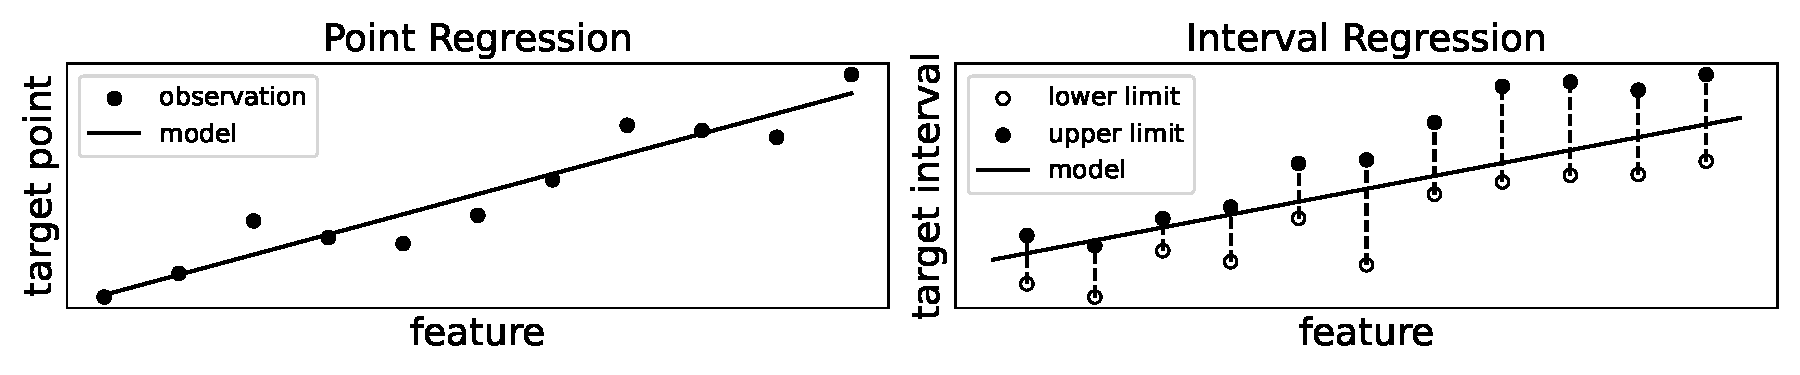
\includegraphics[width=0.99\textwidth]{figs/interval_regression.pdf}
\caption{Example of point regression versus interval regression}
\label{fig:interval_regression}
\end{figure}


\paragraph{Censored Data and Likelihood Function}

In survival analysis, the data may be \textit{right-censored}, meaning the event of interest has not occurred by the end of the study. The likelihood function must account for both observed and censored data.
\newline
\newline
\noindent Let $\delta_i$ be an indicator variable, where:
\[
\delta_i =
\begin{cases}
1 & \text{if the event is observed}, \\
0 & \text{if the observation is censored}.
\end{cases}
\]

\noindent The likelihood function for the AFT model with censored data is:

\begin{equation*}
    L(\boldsymbol{\beta}) = \prod_{i=1}^n \left[ f(T_i \mid \mathbf{x}_i, \boldsymbol{\beta}) \right]^{\delta_i} \left[ S(T_i \mid \mathbf{x}_i, \boldsymbol{\beta}) \right]^{1-\delta_i}
\end{equation*}

where $f(T_i \mid \mathbf{x}_i, \boldsymbol{\beta})$ is the probability density function, and $S(T_i \mid \mathbf{x}_i, \boldsymbol{\beta}) = P(T_i > t)$ is the survival function.
The survival function represents the probability that the event has not occurred by a certain time \( t \), i.e.,
\[
S(T_i \mid \mathbf{x}_i, \boldsymbol{\beta}) = 1 - F(T_i \mid \mathbf{x}_i, \boldsymbol{\beta}),
\]

where \( F(T_i \mid \mathbf{x}_i, \boldsymbol{\beta}) \) is the cumulative distribution function (CDF) of the event time \( T_i \) conditional on the covariates \( \mathbf{x}_i \) and model parameters \( \boldsymbol{\beta} \).
\newline
\newline
\noindent Taking the logarithm of the likelihood function yields the log-likelihood:

\begin{equation*}
    \ell(\boldsymbol{\beta}) = \sum_{i=1}^n \left[ \delta_i \log f(T_i \mid \mathbf{x}_i, \boldsymbol{\beta}) + (1-\delta_i) \log S(T_i \mid \mathbf{x}_i, \boldsymbol{\beta}) \right]
\end{equation*}


\begin{figure}[!t]
\centering
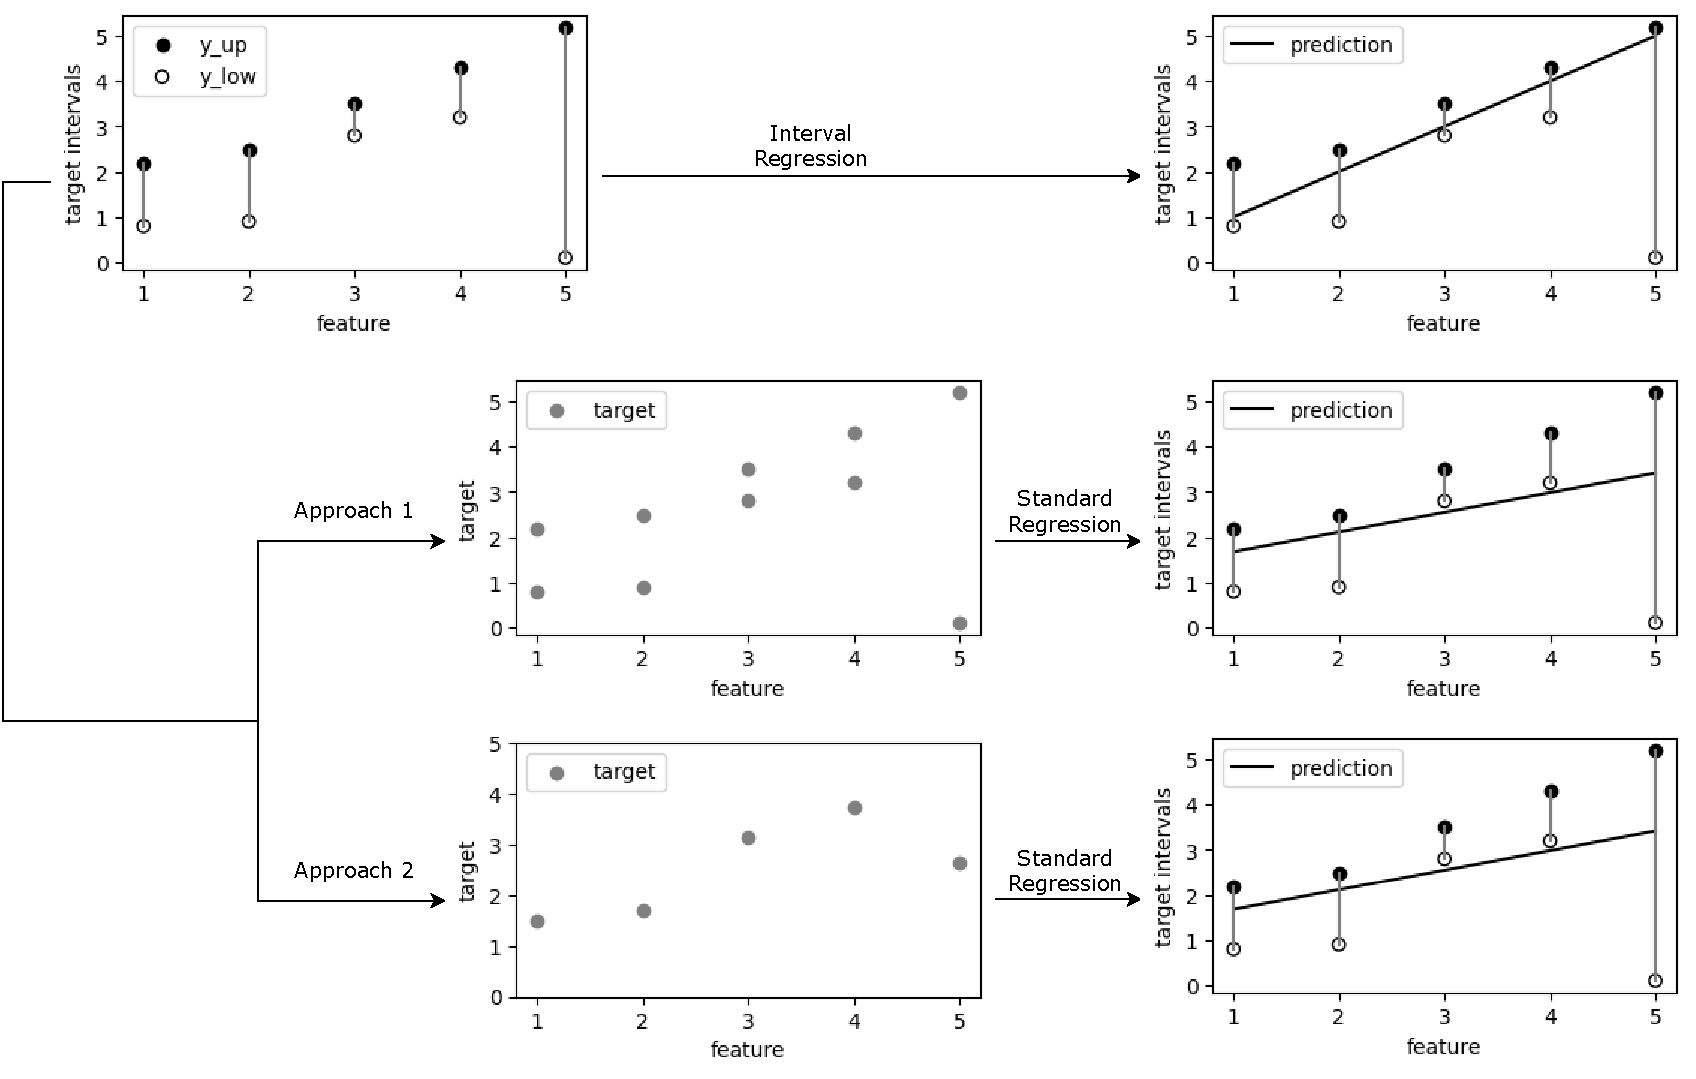
\includegraphics[width=0.99\textwidth]{figs/figs.Convert_Intervals_to_points.pdf}
\caption{Example of converting Interval Regression into Standard Regression}
\label{fig:convert_interval_to_standard}
\end{figure}


\paragraph{Model Fitting Procedure}

To estimate the parameters $\boldsymbol{\beta}$, we maximize the log-likelihood function. The general steps for training the AFT model are:

\begin{enumerate}
    \item Specify the distribution for the error term $\epsilon_i$ (e.g., normal, log-normal, Weibull).
    \item Define the likelihood function based on the observed and censored data.
    \item Maximize the log-likelihood function to estimate $\boldsymbol{\beta}$.
    \item Use the estimated parameters to make predictions.
\end{enumerate}



\paragraph{Example: Survival Analysis with Normal Distribution}

Let us consider the case where the survival times follow a normal distribution, i.e., $\epsilon_i \sim N(0, \sigma^2)$. The model is given by:

\begin{equation*}
    \log(T_i) = \beta_0 + \beta_1 x_{i1} + \epsilon_i, \quad \epsilon_i \sim N(0, \sigma^2)
\end{equation*}

\noindent The corresponding log-likelihood function for this model is:

\begin{equation*}
    \ell(\boldsymbol{\beta}, \sigma) = \sum_{i=1}^n \left[ \delta_i \log \left( \frac{1}{\sigma \sqrt{2 \pi}} \exp\left( -\frac{(\log T_i - \mathbf{x}_i^\top \boldsymbol{\beta})^2}{2 \sigma^2} \right) \right) + (1-\delta_i) \log S(T_i \mid \mathbf{x}_i, \boldsymbol{\beta}, \sigma) \right]
\end{equation*}

where $S(T_i \mid \mathbf{x}_i, \boldsymbol{\beta}, \sigma)$ is the survival function for the normal distribution:

\begin{equation*}
    S(T_i \mid \mathbf{x}_i, \boldsymbol{\beta}, \sigma) = 1 - \Phi\left( \frac{\log T_i - \mathbf{x}_i^\top \boldsymbol{\beta}}{\sigma} \right)
\end{equation*}

and $\Phi(\cdot)$ is the cumulative distribution function (CDF) of the standard normal distribution.
\newline
\newline
\noindent The parameters $\beta_0$, $\beta_1$, and $\sigma$ are estimated by maximizing the log-likelihood function. Predictions for new individuals can be made by:

\begin{equation*}
    \hat{T}_{\text{new}} = \exp(\mathbf{x}_{\text{new}}^\top \hat{\boldsymbol{\beta}} + \hat{\epsilon})
\end{equation*}

where $\hat{\epsilon}$ is drawn from $N(0, \hat{\sigma}^2)$.

\begin{table}[!t] 
\centering
\begin{tabular}{l|l|l|l} 
\toprule
\textbf{model} & \textbf{source code} & \textbf{language} & \textbf{citation} \\ \midrule
linear                 & \citep{penaltyLearning} & R                                      & \citep{rigaill2013penalty}             \\ 
mmit                   & \citep{mmit_package} & C++                     & \citep{mmit}                           \\ 
aft\_xgb               & \citep{xgb_package} & Python                                 & \citep{aft_xgboost}                    \\ \midrule
constant                    & \href{https://github.com/lamtung16/ML_IntervalRegression}{paper GitHub repo} & C++                                 & additional baseline                               \\ \midrule
knn                    & \href{https://github.com/lamtung16/ML_IntervalRegression}{paper GitHub repo} & Python                                 & proposed                               \\ 
mlp                    &\href{https://github.com/lamtung16/ML_IntervalRegression}{paper GitHub repo}& Python                                 & proposed                               \\ 
mmif                   &\href{https://github.com/lamtung16/ML_IntervalRegression}{paper GitHub repo}& C++                     & proposed                               \\ 
\bottomrule
\end{tabular}
\caption{List of the regression models in this with corresponding source.}
\label{tab:models}
\end{table}

\subsubsection{AFT Model in XGBoost}
The AFT model in XGBoost, introduced by \citet{aft_xgboost}, is an ensemble tree-based model designed for survival analysis. 
The model makes predictions as follows:  
\[
y_p = \mathbf{T}(\mathbf{x}),
\]
where $\mathbf{T}$ represents the ensemble of trees in XGBoost.
Although it belongs to the AFT model family, this model can handle all non-negative target intervals.
To extend its applicability to real-valued target intervals $(y_l, y_u) \in \mathbf{R}^2$, \citet{aft_xgboost} apply an exponential transformation to the original interval:  
\[
(y_l, y_u) \longrightarrow (\exp y_l, \exp y_u) \in \mathbf{R}_{+}^2
\]
After making a prediction $y_p$ in the exponential space, the result is mapped back to the original scale using the logarithm transformation:
\[
\hat{y} = \log y_p = \log \mathbf{T}(\mathbf{x})
\]

Training this model is based on minimizing the negative log-likelihood function (loss function), which incorporates all training survival instances:

\begin{equation} \label{eq:aft_loss}
    l_{AFT}\Big(\hat{y}, (y_l, y_u)\Big) = -\log \Big[ F_Z\big( \frac{y_u - \hat{y}}{\sigma} \big) - F_Z\big(\frac{y_l - \hat{y}}{\sigma}\big) \Big]
\end{equation}



\noindent where $\sigma > 0$ is the scale parameter.
The cumulative distribution function $F_Z(z)$ depends on the chosen distribution (normal, logistic, or extreme):
\begin{itemize}
    \item normal: \phantom{00}   $F_Z(z) = \frac{1}{2}\big( 1 + \text{erf}(\frac{z}{\sqrt{2}}) \big)$
    \item logistic: \phantom{00} $F_Z(z) = \frac{e^z}{1+e^z}$
    \item extreme: \phantom{0} $F_Z(z) = 1 - e^{-\exp z}$
\end{itemize}

Figure \ref{fig:aft_loss_func} visualizes the loss function for each distributions, which can be compared to Figure \ref{fig:loss_func} to observe their similarities. 
The model is trained using the gradient boosting algorithm \citep{gradient_boosting} to minimize the loss value \eqref{eq:aft_loss} over the training dataset with $N$ instances $\{\mathbf{x}^i, (y_l^i, y_u^i)\}_{i=1}^N$ given the distribution and the scale parameter $\sigma$:
\begin{equation*}
    \sum_{i = 1}^N l_{AFT}\Big(\hat{y}^i, (y_l^i, y_u^i)\Big) = \sum_{i=1}^N -\log \Big[ F_Z\big( \frac{y_u^i - \log\mathbf{T}(\mathbf{x}^i)}{\sigma} \big) - F_Z\big(\frac{y_l^i - \log\mathbf{T}(\mathbf{x}^i)}{\sigma}\big) \Big]
\end{equation*}

\begin{figure}[!t]
\centering
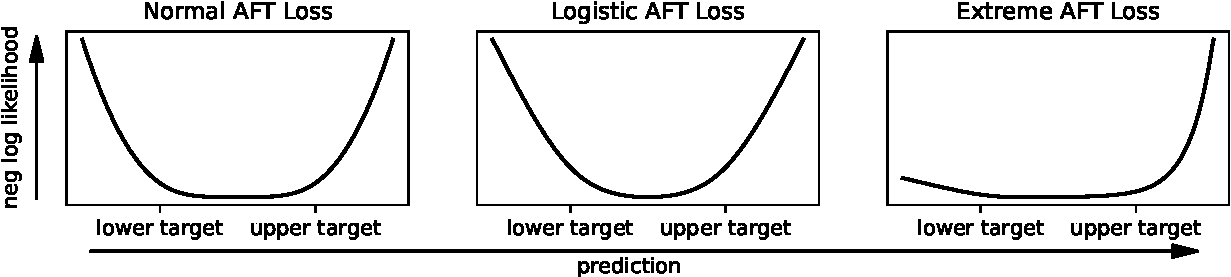
\includegraphics[width=0.99\textwidth]{figs/fig.aft_loss_function.pdf}
\caption{Visualization of the AFT XGBoost Loss (negative log-likelihood) for 3 distributions}
\label{fig:aft_loss_func}
\end{figure}

\subsection{Supervised Machine Learning Models}

Before delving into the methods, it is essential to clarify the loss function that these models utilized in interval regression.
While the mean squared error (MSE) or mean absolute error (MAE) is commonly used for traditional regression tasks, interval regression employs a related criterion known as hinge error. 
The hinge loss function, leveraging the ReLU activation function, is defined as:
\begin{equation}\label{eq:loss_func}
l(\hat{y}, y) = l(\hat{y}, [y_l, y_u]) = \big( \text{ReLU}(y_{l} - \hat{y} + \epsilon)\big)^p + \big(\text{ReLU}(\hat{y} - y_{u} + \epsilon) \big)^p
\end{equation}
where $\epsilon \geq 0$ is the margin (or hinge), $\hat{y}$ denotes the predicted value and $y = [y_l, y_u]$ represents the target interval with $y_l \leq y_u$.
$p$ is either 1 or 2 ($p=1$ is equivalent to MAE, $p=2$ is equivalent to MSE).
This formulation ensures that the loss is minimized when the predicted value $\hat{y}$ falls within the target interval $[y_l, y_u]$.
Unlike MSE or MAE, which achieves zero loss at a single target value, the hinge error function yields zero loss within a specified target interval, as illustrated in Figure \ref{fig:loss_func}.

From this point forward in the study, the following notation will be used: $\textbf{x}$ represents the feature vector, $[y_l, y_u]$ denotes the target interval, and $\hat{y}$ stands for the predicted output.

\begin{figure}[!t]
\centering
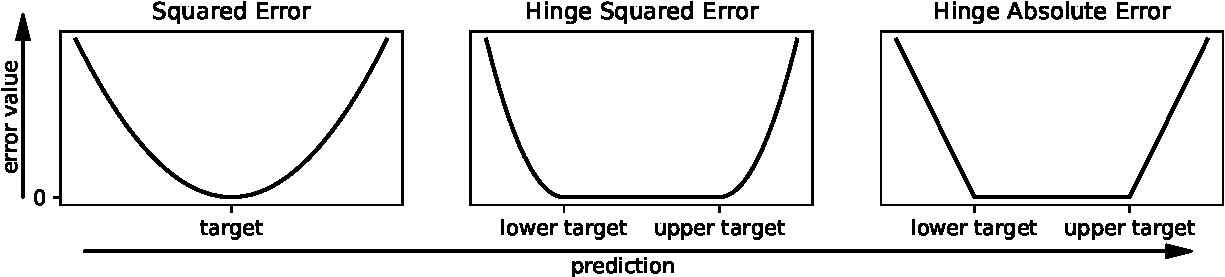
\includegraphics[width=0.99\textwidth]{figs/figs.loss_function.pdf}
\caption{Visualization of the Loss Functions: Error values relative to predictions and targets}
\label{fig:loss_func}
\end{figure}

\subsubsection{Linear}
This linear model was introduced in the first time by \citet{rigaill2013penalty}, and its extended theoretical foundations were later studied by \citet{rit}.
The prediction formula is given:
\begin{equation} \label{eq:linear_prediction}
    \hat{y} = \mathbf{x} \cdot \beta + \beta_0
\end{equation}
where $\beta \in \mathbf{R}^m$ and $\beta_0 \in \mathbf{R}$ are the parameters to be learned. To estimate these parameters, the authors extended the Standard Regression loss function—specifically, the Squared Error or Mean Squared Error (MSE)—into a generalized form called the \textit{Hinge Squared Error}.
The error value between prediction $\hat{y}$ and target interval $(y_l, y_u)$ is defined as follows: 

$$l\Big(\hat{y}, (y_l, y_u)\Big) = 
\begin{cases} 
    (y_l - \hat{y} + \epsilon)^2, & \mbox{if } \hat{y} < y_l + \epsilon \\
    0, & \mbox{if } y_l + \epsilon \leq \hat{y} \leq y_u - \epsilon \\
    (\hat{y} - y_u + \epsilon)^2, & \mbox{if } \hat{y} > y_u - \epsilon
\end{cases}$$

\noindent where $\epsilon \geq 0$ is the margin length ($\epsilon=0$ by default).
The loss function becomes MSE when $y_l = y_u$ and $\epsilon = 0$, or in other word, target interval becomes target point.

\citet{rit} proposed a model called \textit{Regression with Interval Targets} (RIT), which is essentially the same as model \eqref{eq:linear_prediction}, but uses \textit{Hinge Absolute Error} instead:

$$l\Big(\hat{y}, (y_l, y_u)\Big) = 
\begin{cases} 
    |y_l - \hat{y} + \epsilon|, & \mbox{if } \hat{y} < y_l + \epsilon \\
    0, & \mbox{if } y_l + \epsilon \leq \hat{y} \leq y_u - \epsilon \\
    |\hat{y} - y_u + \epsilon|, & \mbox{if } \hat{y} > y_u - \epsilon
\end{cases}$$

\noindent The general Interval Regression loss function can be written in this short form:

\begin{equation} \label{eq:lossfunction}
    l\Big(\hat{y}, (y_l, y_u)\Big) = \Big( \text{ReLU}(y_l - \hat{y} + \epsilon)\Big)^p + \Big(\text{ReLU}(\hat{y} - y_u + \epsilon) \Big)^p
\end{equation}

\noindent where $p \in \{1, 2\}$. Refer to Figure \ref{fig:loss_func} for the visual comparison between hinge errors (Interval Regression Loss) and squared error (Standard Regression Loss).

To estimate the parameters $\beta$ and $\beta_0$ in \eqref{eq:linear_prediction}, apply a gradient descent algorithm with respect to $\beta$ and $\beta_0$ to minimize the Hinge Error \eqref{eq:lossfunction} over the training dataset having $N$ instances $\{\mathbf{x}^i, (y_l^i, y_u^i)\}_{i=1}^N$:
\begin{equation*}
    \sum_{i = 1}^N l\Big(\hat{y}^i, (y_l^i, y_u^i)\Big) = \sum_{i = 1}^N l\Big(\mathbf{x^i} \cdot \beta + \beta_0, (y_l^i, y_u^i)\Big)
\end{equation*}
\citet{rigaill2013penalty} employed the Fast Iterative Shrinkage-Thresholding Algorithm or FISTA \citep{fista}, while \citet{rit} employed stochastic gradient descent (SGD).

\subsubsection{Tree} MMIT introduced by \citet{mmit} is applicable for $\lambda$ prediction as an interval regression model. 
The MMIT model is:
\[
\log \hat{\lambda} = \mathcal{T}(\mathbf{x})
\]
The tree $\mathcal{T}$ architecture follows the same structure as CART (Classification And Regression Tree) \citep{cart}. 
The only difference lies in the regression value for each leaf which is a set of $Q$ instances $\{\mathbf{x}^i, [\log \lambda_l^i,\log \lambda_u^i]\}_{i=1}^Q$: instead of taking the mean of all targets like CART does, it chooses a constant value $c$ that minimizes the mean Hinge Error \eqref{eq:loss_func} between this constant and the target intervals:
\begin{equation*}
    \argmin_c \frac{1}{Q} \sum_{i=1}^{Q} l\big(c, [\log \lambda_l^i, \log \lambda_u^i]\big), \quad c \in \mathbf{R}
\end{equation*}
\noindent A heuristic algorithm is used to speed up the estimation of the mean value for each leaf by considering a finite set of candidates, rather than solving for the optimal $c$:
\begin{align*}
    &\argmin_c \frac{1}{Q} \sum_{i=1}^{Q} l\big(c, [\log \lambda_l^i, \log \lambda_u^i]\big), 
    \\
    &\text{where }c \in \{\log \lambda_l^i, \log \lambda_u^i, \frac{\log \lambda_l^i + \log \lambda_u^i}{2}|\log \lambda_l^i > -\infty, \log \lambda_u^i < \infty\}_{i = 1}^Q
\end{align*}

\noindent The training procedure for determining the optimal tree architecture follows the same operations as in CART (binary optimization) to minimize the Hinge Error \eqref{eq:loss_func} over the train dataset having $S$ instances $\{\mathbf{x}^i, [\log \lambda_l^i, \log \lambda_u^i]\}_{i=1}^S$:
\begin{equation*}
    \sum_{i = 1}^S l\Big(\log \hat{\lambda}^i, [\log \lambda_l^i, \log \lambda_u^i]\Big) = \sum_{i = 1}^S l\Big(\mathcal{T}(\mathbf{x}^i), [\log \lambda_l^i, \log \lambda_u^i]\Big)
\end{equation*}
The optimal tree architecture (maximum depth, minimum split), loss type  which is $p$ (either 1 or 2) in Hinge Error \eqref{eq:loss_func}, and margin which is $\epsilon$ in Hinge Error \eqref{eq:loss_func}, is selected through cross-validation.


\newpage

\begin{figure}[!t]
\centering
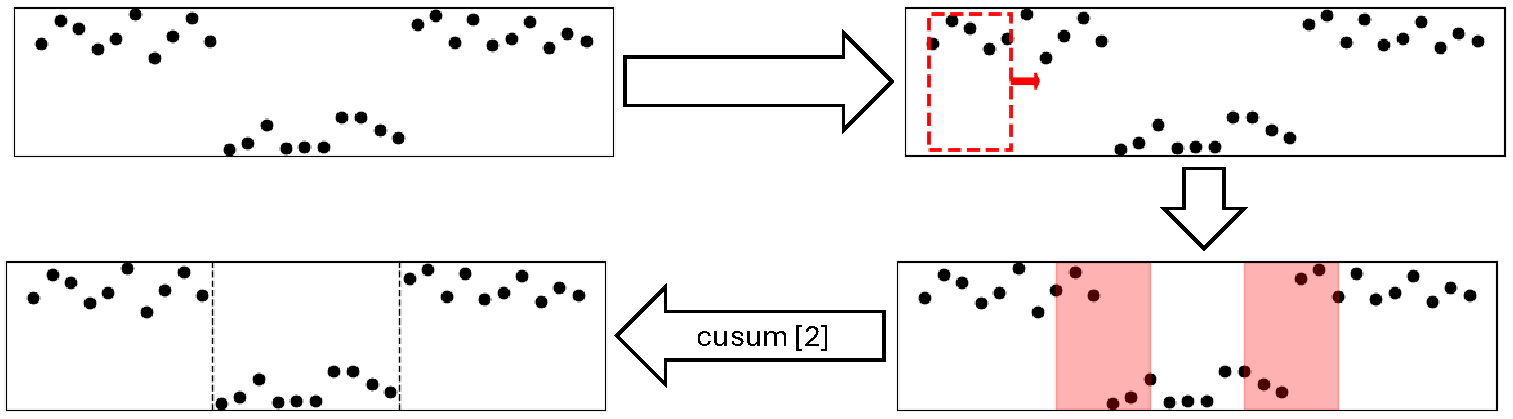
\includegraphics[width=0.99\textwidth]{figs/fig.DL_cdp}
\caption{Changepoint detection using Deep Learning}
\label{fig:cdp_DL}
\end{figure}

\section{Literature Review: Optimal Partitioning}
\subsection{Changpoint Detection Algorithms}
Changepoint detection serves as a vital tool in numerous real-life applications by pinpointing significant transitions or sudden changes in data patterns, ranging from detecting market trends in finance \citep{app:finance}, monitoring disease outbreaks in healthcare \citep{cancer}, enhancing network security \citep{app:network}, monitoring environmental changes \citep{app:climate} and more.

Changepoint detection methods can be divided into two categories: Deep Learning (DL) and Dynamic Programming (DP).
DL-based methods, which inspired from a statistical method Cumulative Sum (CUSUM) \citep{review:cusum, review:james1987tests}, including recent works \citep{review:li24automatic, review:ermshaus2023clasp} employ multilayer perceptrons (MLP) or k-nearest neighbors (KNN) as classification sliding windows to identify changepoints. 
Take a look at the Figure \ref{fig:cdp_DL} for a clear visualization of the operation.
However, these methods rely on local neighbors rather than the entire sequence and are overly complex for univariate data.
In contrast, DP is well-suited for this context.

To determine the optimal partition of a sequence given a fixed number of segments (or number of changepoints), several efficient algorithms can be employed to achieve precise results \citep{auger1989algorithms, bai2003computation, killick2012optimal}. 
However, in many instances, the number of segments is not predetermined and must instead be inferred from the data. 
To address this challenge, several dynamic programming algorithms have been successfully applied to changepoint detection, including Optimal Partitioning (OPART) \citep{jackson:05} with its variations such as Pruned Exact Linear Time (PELT) \citep{killick2012optimal} or Functional Pruning Optimal Partitioning (FPOP) \citep{Maidstone:16}.
PELT uses a theorem to prune certain candidate changepoints that cannot be part of the optimal partition. 
FPOP prunes at least as many candidate changepoints as PELT and can be more efficient, particularly for large datasets. 
Despite these differences, OPART, PELT, and FPOP all produce the same partition.
The Labeled Optimal Partitioning (LOPART) \citep{hocking:20} extends OPART's capabilities by leveraging predefined changepoint labels, indicating the expected number of changepoints within specific location ranges.
When no such labels are defined, LOPART behaves identically to OPART.
Without prior knowledge of the number of changepoints in the partition and aiming to limit their occurrence, these algorithms employ a penalty parameter to discourage the presence of changepoints, denoted as $\lambda$, in the following optimization problem

\begin{figure}[!t]
\centering
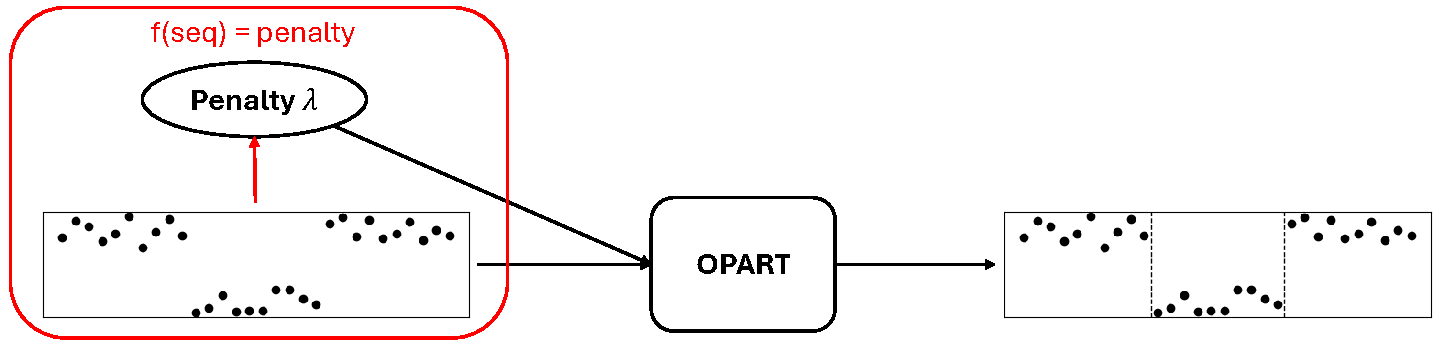
\includegraphics[width=0.99\textwidth]{figs/fig.overall_focus}
\caption{The challenge of using OPART is predicting the value for penalty}
\label{fig:focus}
\end{figure}

\paragraph{OPART problem} Find partition vector $\mathbf{m} \in \mathbb{R}^N$ that minimizes the following cost function for a given sequence $\mathbf{d} \in \mathbb{R}^N$ and penalty parameter $\lambda \geq 0$:
\begin{align}
\textbf{m} &= \underset{\textbf{m}}{\text{argmin}} \ C_\lambda(\textbf{d}, \textbf{m}) \\
\text{where} \quad C_\lambda(\textbf{d}, \textbf{m}) &= \sum_{i=1}^N l(d_i, m_i) + \lambda I[m_i \neq m_{i+1}]
\end{align}

\noindent where $l(m_i, d_i)$ usually represents the squared error between the sequence value $d_i$ and the mean segment $m_i$, i.e., $l(d_i, m_i) = (m_i-d_i)^2$.
$I[m_i \neq m_{i+1}]$ is an indicator function that equals 1 if there is a changepoint (when $m_i \neq m_{i+1}$) and 0 otherwise. 
Thus, $k = \sum_{i=1}^N I[m_i \neq m_{i+1}]$ represents the total number of changepoints, hence $k+1$ is the number of segments.
For instance, for a sequence $\textbf{d} = [d_1, d_2, d_3, d_4, d_5, d_6] \in \mathbb{R}^{6}$, if we have a fixed penalty $\lambda^*$, the optimal partition vector of problem \ref{eq:opart_loss} is $\textbf{m} = [m_1, m_1, m_1, m_1, m_2, m_2]$ , this indicates that the partition $\textbf{m}$ consists of 1 changepoint and 2 segments: $[d_1, d_2, d_3, d_4]$ and $[d_5, d_6]$.


\begin{figure}[!t]
\centering
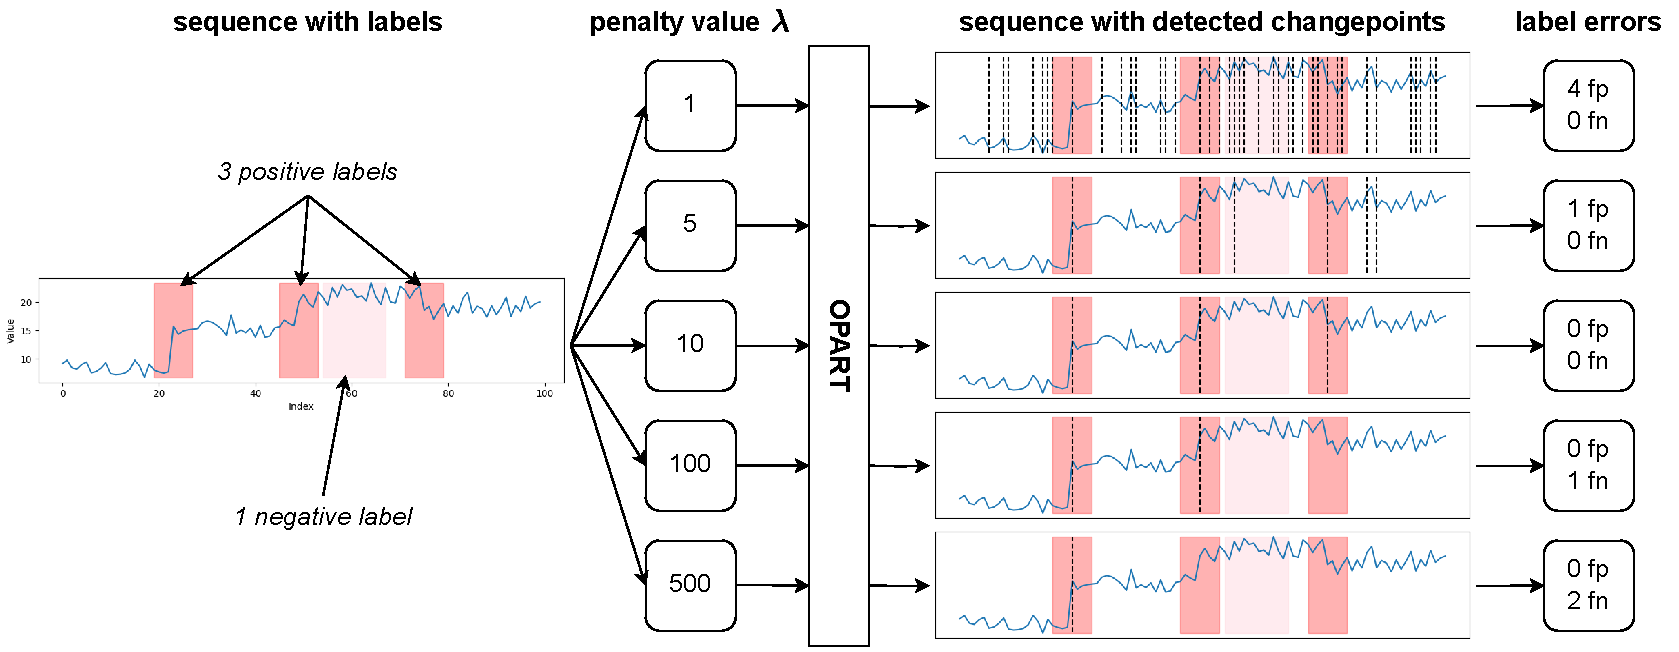
\includegraphics[width=0.99\textwidth]{figs/fig.lambdachanging.pdf}
\caption{Different penalty result in varied sets of changepoints}
\label{fig:lambda}
\end{figure}


\paragraph{Role of the penalty parameter $\lambda$} Within the OPART problem \ref{eq:opart_loss}, the penalty parameter $\lambda$ holds significant importance in partitioning.
Moreover, a higher $\lambda$ imposes a more substantial penalty for changepoints' presence, consequently yielding smaller sets of changepoints.
When $\lambda = 0$, the optimal partition $\textbf{m}$ in problem \ref{eq:opart_loss} matches the given sequence $\textbf{d}$ exactly ($\textbf{m} \equiv \textbf{d}$), while as $\lambda$ approaches $+\infty$, all values in $\textbf{m}$ is the mean of $\textbf{d}$.
A too high value of $\lambda$ is undesirable because it results in fewer detected changepoints, potentially missing significant ones.
Conversely, a too low value of $\lambda$ results in an excessive number of detected changepoints, more than necessary.
While the existing changepoint detection algorithms has demonstrated effectiveness, the fixed nature of $\lambda$ prompts inquiry into methods for dynamically adapting this critical parameter.



\subsection{Relationship between OPART and Interval Regression}\label{subsec:problem_setting}
OPART algorithms take into the sequence $\mathbf{d}$ along with $\lambda$ as input to generate the set of detected changepoints.
Each labeled sequence $\textbf{d}^j$ has $M_j$ distinct labels $\{(s_i, e_i, c_i)\}_{i=1}^{M_j}$, where \( c_i \) denotes the expected number of changepoints between start location \( s_i \) and end location \( e_i \).
There are two types of label errors: in each label, if the number of detected changepoints greater than \( c_i \), it's a \textit{false positive}; if smaller, it's a \textit{false negative}.

\begin{figure}[!t]
\centering
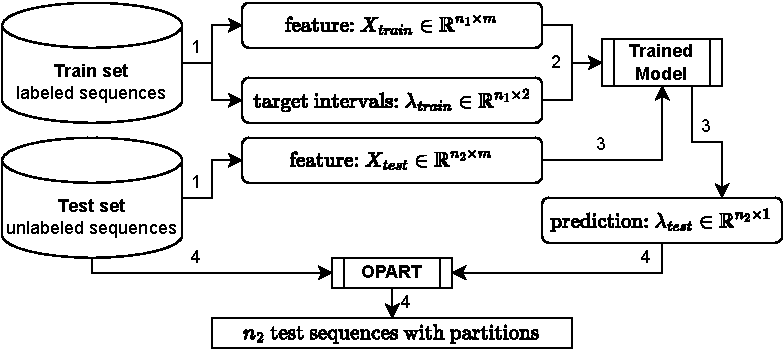
\includegraphics[width=0.99\textwidth]{figs/fig.problem_setting.pdf}
\caption{The process involves a labeled sequences train set and a unlabeled sequences test set}
\label{fig:problem_setting}
\end{figure}

Finding the optimal partition for a given labeled sequence require considering a range of values for $\lambda$ (rather than just one specific value) that minimizes the number of label errors.
Refer to \citep{rigaill2013penalty} for a method to determine the optimal range of \(\lambda\) for each labeled sequence.
Consequently, the value of $\lambda$ to be predicted should fall within an optimal interval, see Figure \ref{fig:interval_regression}.
This type of problem, where the objective is to find values falling within an interval, is referred to as the \textit{interval regression}.

\newpage
\section{Literature Gaps and Proposed Plans}
\subsection{Inteval Regression}
\paragraph{Limitation} Let me briefly summarize the previous works and highlight their limitations:
\begin{itemize}
    \item \textbf{Original AFT model and its variants}: Designed for survival analysis, it handles only uncensored and right-censored data, as it does not account for left-censored data.
    \item \textbf{AFT model in XGBoost}: Capable of handling all types of censored data by transforming target intervals to ensure non-negative values. It introduces a loss function for all types of censored outcomes. However, being tree-based, the model lacks smooth decision boundaries.
    \item \textbf{Linear model in supervised machine learning}: Similar to the original AFT model, it has a simple linear architecture that struggles with datasets exhibiting non-linear patterns.
    \item \textbf{MMIT}: A non-linear model that captures complex relationships, but like any tree-based models, it produces non-smooth decision boundaries, leading to a lack of smoothness in predictions.
\end{itemize}

\paragraph{Proposed Plan} My plan involves utilizing more sophisticated and smoother models, such as Generalized Additive Models (GAMs) \citep{hastie2017generalized}, random forest, or like multi-layer perceptrons (MLP). 
\begin{itemize}
    \item One option would be an MLP with just one hidden layer and very few neurons, using Rectified Linear Unit activation functions like ReLU or Leaky ReLU (not ELU or SELU or anything that creates non-linear regions). For instance, an MLP with one hidden layer and two neurons, using Leaky ReLU as the activation function, can be about twice as complex as a linear model, as it can create up to four linear regions (see Proposition 3 in \citep{montufar2014number}). This makes it a more general approach than traditional linear models without being overly complex.
    
    \item Alternatively, for a non-linear model that remains relatively simple, I could opt for piecewise linear models, like splines \citep{friedman1991multivariate} with linear terms in each region.
    

\end{itemize}



\subsection{Changepoint Detection}
\paragraph{Limitation} The OPART algorithm employs a fixed penalty value, $\lambda$, which may limit its adaptability to different data structures.
\paragraph{Proposed Plan}
\begin{itemize}
    \item Explore heuristic approaches that divide the data into smaller segments, followed by applying optimal partitioning to each subsequence.
    \item Consider applying k-means clustering to detect potential segments.
    \item Applying complex models for penalty prediction.
\end{itemize}



\newpage

\begin{figure}[!t]
\centering
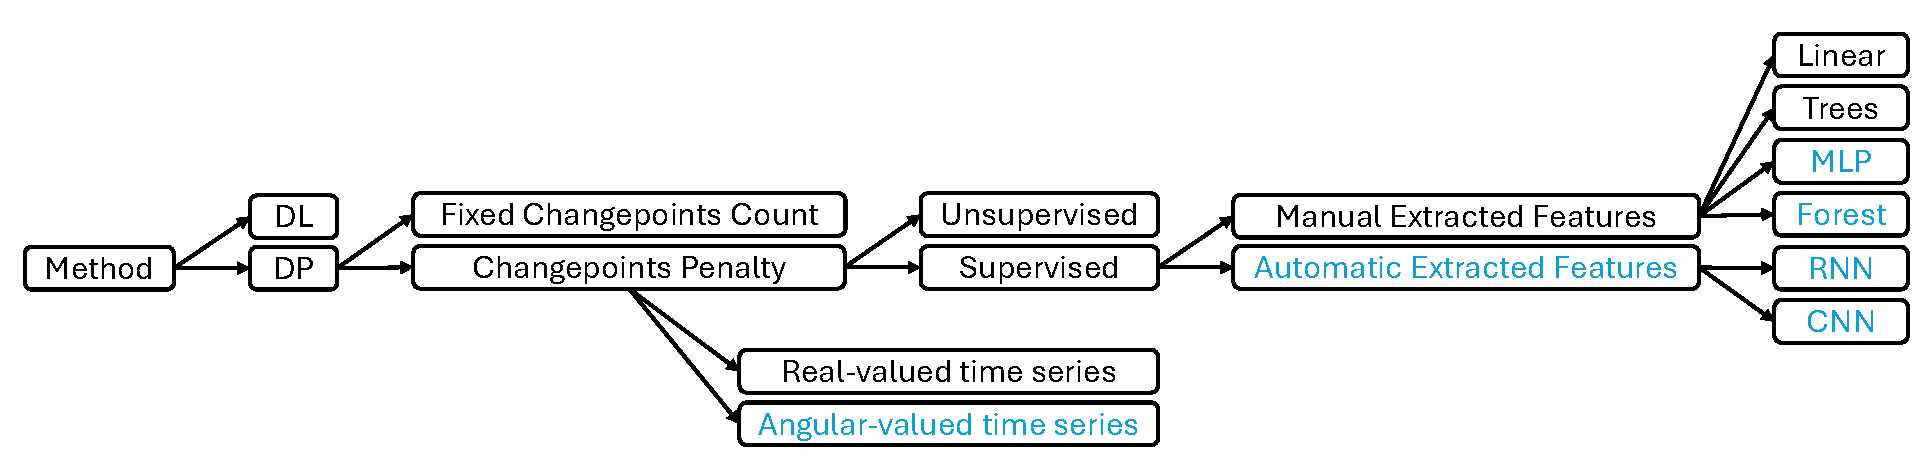
\includegraphics[width=0.99\textwidth]{figs/comprehensive}
\caption{Comprehensive Diagram: Review and Contributions}
\label{fig:comprehensive}
\end{figure}

\section{My Contributions}

\subsection{Optimal Partitioning Penalty Learning: MLP}
Changepoint detection (or other words, partitioning and segmentation) is essential in many real-world applications, identifying significant data shifts in finance \citep{app:finance}, healthcare \citep{cancer}, network security \citep{app:network}, environmental monitoring \citep{app:climate}, and more.

Detecting changepoints involves selecting the detection method and tuning hyperparameters to detect the changepoint locations.

\paragraph{Changepoint detection methods review}
Many real-life time series data are univariate.
Several deep learning (DL)-based changepoint detection methods exist \citep{review:londschien2023randomforest, review:lee2023, review:li24automatic, review:ermshaus2023clasp}, these approaches generalize classical methods \citep{review:cusum, review:james1987tests} by applying sliding classification windows built using either multilayer perceptron (MLP) or k-nearest neighbors (KNN). 
DL-based methods are fairly easy to understand and implement, making them accessible to a wide audience.
But these methods require tuning numerous hyperparameters, making them overly complex for univariate data.
In contrast, dynamic programming (DP) algorithms provides an ideal solution in this context.
\textit{This study selects DP to enhance its changepoint detection performance.}

\paragraph{Regularization for Changepoints Count in DP Algorithms}
DP algorithms detects changepoints using only one hyperparameter (contrast to numerous hyperparameters in DL-based methods) to control changepoints count, either (a) a fixed changepoints count or (b) a penalty to penalize changepoint presence.
Approach (a), used in \citep{auger1989algorithms, bai2003computation, killick2012optimal}, is effective but relies on often unknown changepoints count.
Approach (b), with the most popular methods being Optimal Partitioning (OP) \citep{jackson:05} and its variants, including Pruned Exact Linear Time (PELT) \citep{killick2012optimal}, Functional Pruning Optimal Partitioning (FPOP) \citep{Maidstone:16}, and Labeled Optimal Partitioning (LOP) \citep{hocking:20}.
PELT and FPOP improves efficiency by pruning technique whilst producing the same solution as OP. 
LOP extends OP by incorporating predefined changepoint labels and defaults to OP when labels are absent.
\textit{This study selects approach (b) to enhance changepoint detection performance as it offers greater flexibility.}

\begin{figure}[!t]
\centering
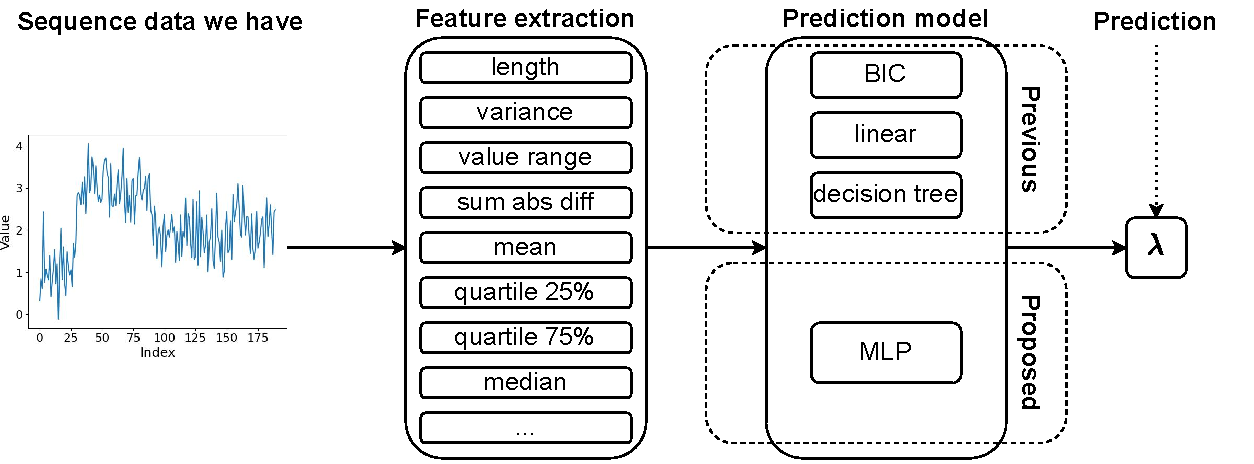
\includegraphics[width=0.9\textwidth]{figs/fig.model_diagram}
\caption{Comparative Model Diagram - Previous Methods versus Our Proposal}
\label{fig:proposed_model}
\end{figure}

\paragraph{The role of the OP penalty}
A higher penalty imposes stricter penalties, reducing the changepoints count (see Figure \ref{fig:lambda}).
Given the suitability of OP family algorithms for changepoint detection in univariate sequences and the role of the OP penalty, \textit{this study focuses on developing a model to predict the optimal OP penalty}.

\paragraph{Related Work review} Various methods exist for predicting the OP penalty, including unsupervised \citep{bic, aic, lavielle05} and supervised ones \citep{truong17, rigaill:13, mmit, aft_xgboost}.

\paragraph{Gap in the Literature and Contributions}  
Existing models are constrained by simplistic architectures, such as linear or tree-based, which motivated us to propose a novel approach. 
This study proposes MLP with activation function ReLU for OP penalty prediction. 
This is a generalized version of a linear model and offers continuous nonlinear predictions compared to tree-based models. 
Experiments conducted on three large genome datasets demonstrate that the proposed model outperforms previous work in accuracy and F1 score.
For simplicity, we refer to the OP penalty as $\lambda$ hereafter.

\begin{figure}[!t]
\centering
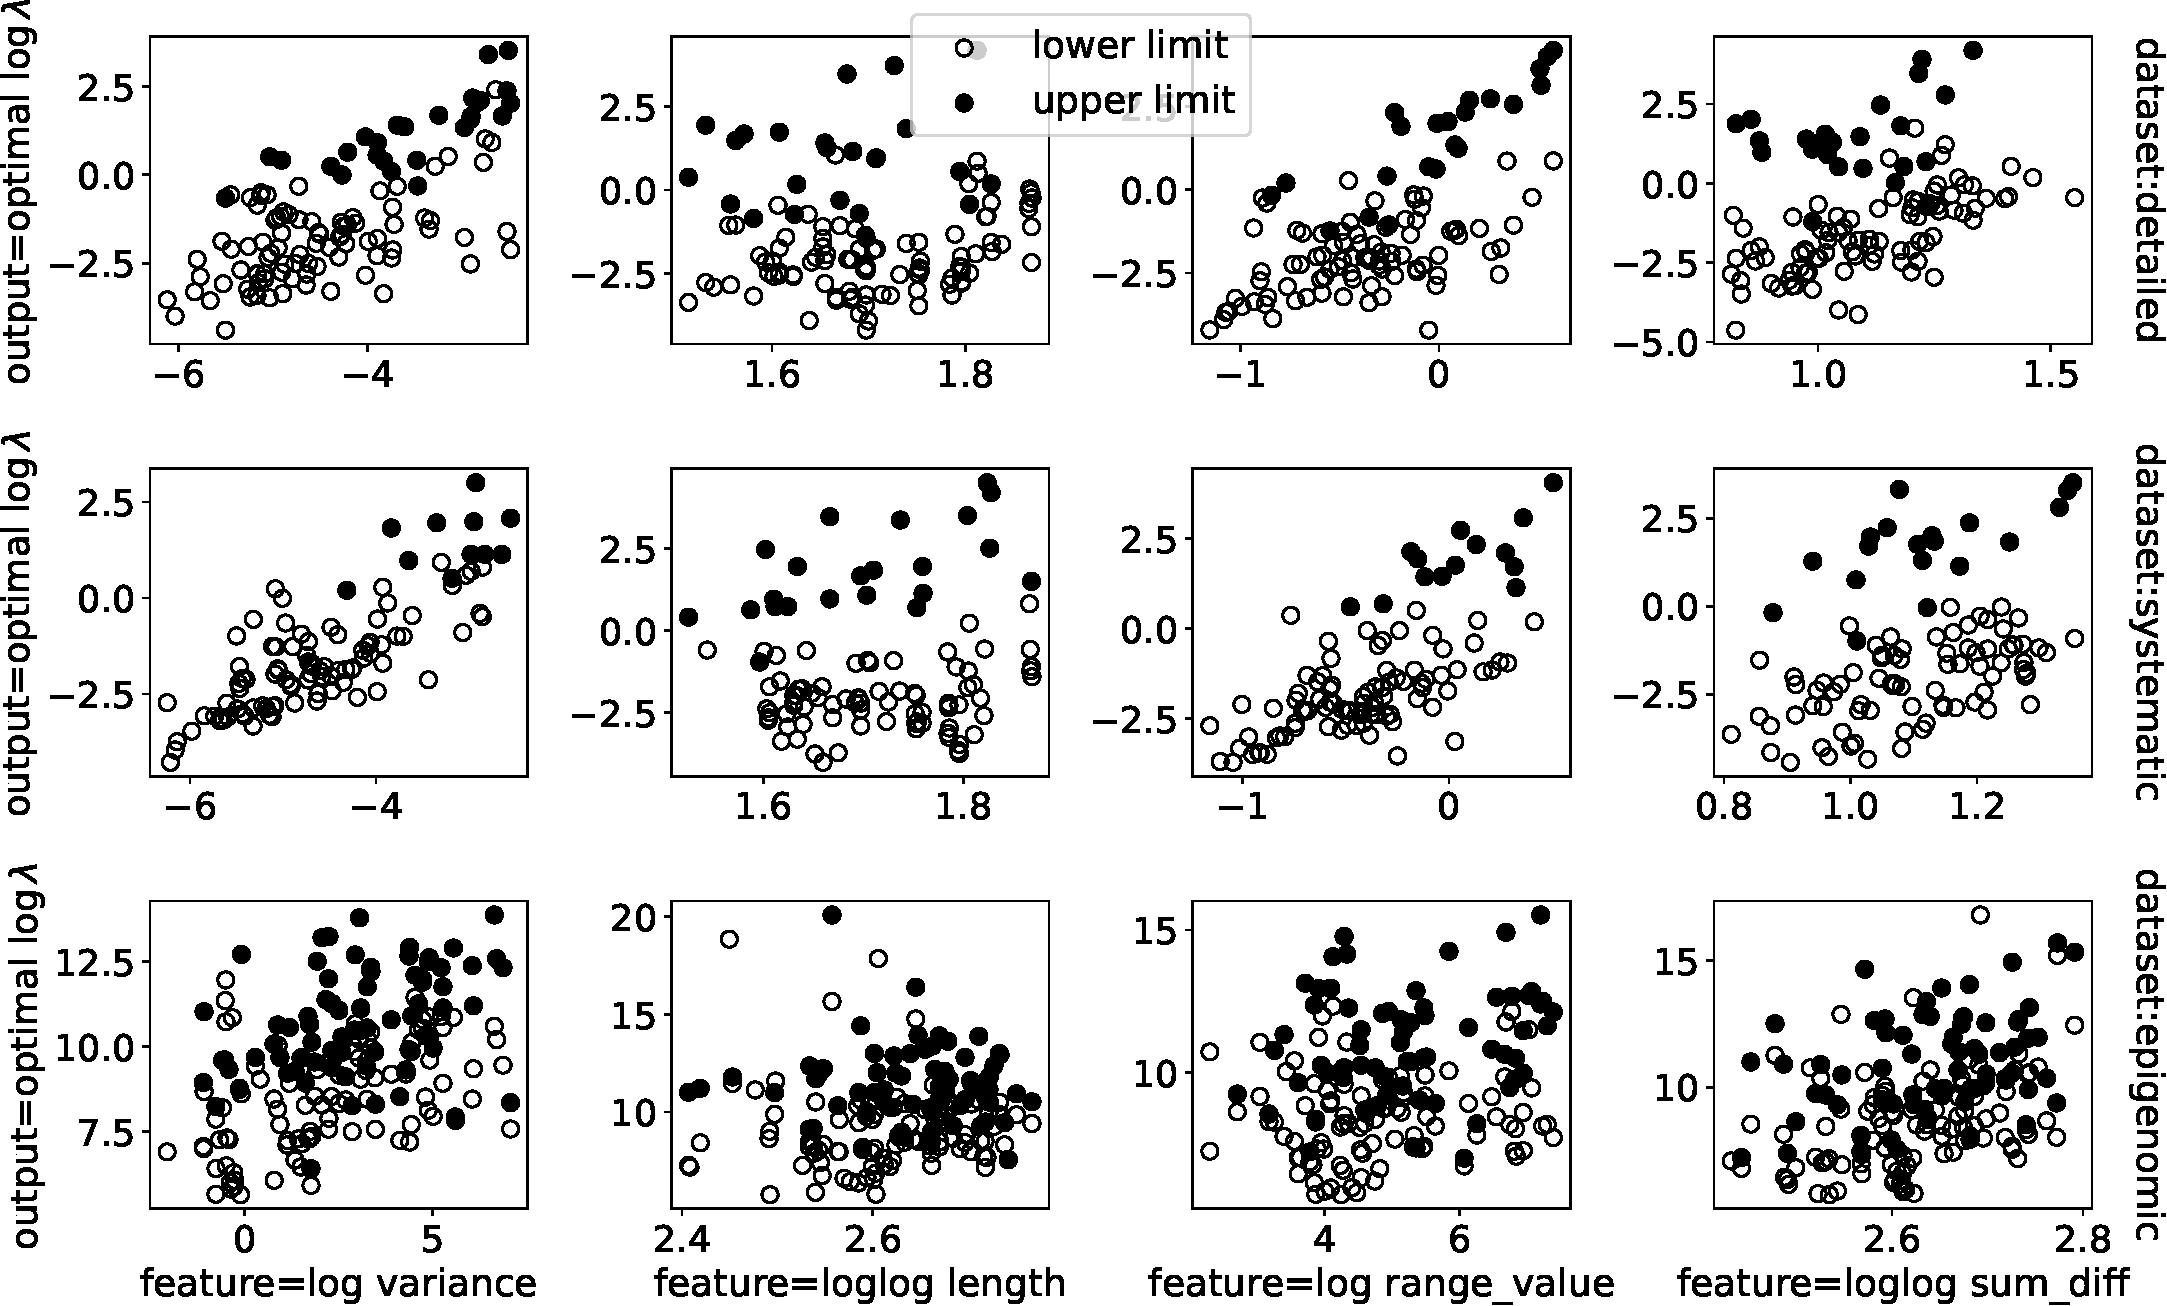
\includegraphics[width=0.95\textwidth]{figs/fig.features_targets_all_datasets}
\caption{Graphs showing the relationship between four features and target intervals}
\label{fig:features_targets}
\end{figure}


\begin{table}[!t]
\centering
\label{tab:list_models}%
\begin{tabular}{@{}lllll@{}}
\toprule
\textbf{Model} & \textbf{Features} & \textbf{Model Type} & \textbf{Regularization} & \textbf{Citation} \\
\midrule
BIC.1 & 1 & unsupervised & None & \cite{bic} \\
\midrule
linear.1 & 1 & \multirow{3}{*}{linear} & \multirow{3}{*}{None} & \multirow{3}{*}{\begin{tabular}[c]{@{}l@{}}\cite{hocking:20}\\ \cite{rigaill:13}\\ \cite{lavielle05}\end{tabular}} \\
linear.2 & 2 &  &  & \\
linear.4 & 4 &  &  & \\
\midrule
linear.all & 118 &  & L1 & \cite{rigaill:13} \\
\midrule
mmit.1 & 1 & \multirow{4}{*}{tree} & max depth & \multirow{4}{*}{\cite{mmit}} \\
mmit.2 & 2 &  & min split sample & \\
mmit.4 & 4 &  & loss type & \\
mmit.all & 118 &  & loss margin & \\
\midrule
 &  &  & distribution scale & \\
aft\_xgboost.1 & 1 & \multirow{4}{*}{ensemble tree} & learning rate & \multirow{6}{*}{\cite{aft_xgboost}} \\
aft\_xgboost.2 & 2 &  & max depth & \\
aft\_xgboost.4 & 4 &  & min child weight & \\
aft\_xgboost.all & 118 &  & reg alpha & \\
 &  &  & reg lambda & \\
\midrule
mlp.1 & 1 & \multirow{4}{*}{MLP} & hidden layers count & \multirow{4}{*}{proposed} \\
mlp.2 & 2 &  & neurons per layer & \\
mlp.4 & 4 &  & early stopping & \\
mlp.all & 118 &  &  & \\
\bottomrule
\end{tabular}
\caption{List of employed penalty prediction models}
\end{table}



\subsubsection{Contribution}
\paragraph{Novelty: MLP for $\lambda$ prediction}
A MLP with fully connected architecture is used.
All hidden layers have the same number of neurons.
ReLU activation function is used in the input and hidden layer(s). This architecture makes the proposed model a more general form of a linear model and produces continuous nonlinear predictions compared to tree-based models like MMIT and AFT in XGBoost.

\paragraph{Additional Contribution: Feature Selection}
A meaningful feature distinguishes sequences from one another in the context of changepoint detection.
Features such as the mean, quartile values (min, Q1, Q2, Q3, max) and their transformations are not selected because these features are noise in the changepoint context.
For example, \([0,0,0,1,1,1]\) and \([1,1,1,2,2,2]\) are the same sequences.
Sequence length and variance alone cannot fully represent a sequence, since some sequences may have the same length and variance but differ significantly in this context, so we introduce two additional sequence-related features: \textit{value range} and \textit{sum of absolute differences}.
\begin{itemize}
\item \textbf{Value range:} This feature ($r$ in Table \ref{tab:models}) is defined as the difference between the maximum and minimum values in the sequence.
\item \textbf{Sum of absolute differences:} This feature ($s$ in Table \ref{tab:models}) is calculated as the sum of the absolute differences between two consecutive sequence points, denoted as $\sum_{i=1}^{N-1} |d_{i+1} - d_{i}|$, where $\textbf{d} = [d_1, d_2, \dots, d_N]$ is the sequence. This feature differentiates sequences with the same length, variance, or value range, such as [0,0,0,1,1,1] and [0,1,0,1,0,1], which are distinct in the context of changepoint detection.
\end{itemize}
Intuitively, as the value range or the sum of absolute differences increases, the sequence tends to show more fluctuations, indicating a need to increase $\lambda$.
See Figure \ref{fig:features_targets} to see why these two features emerge as strong candidates.

I employed cross-validation to determine the appropriate MLP architecture, which was time-consuming, for details, see Figure \ref{fig:mlp}.
My approach achieved improved accuracy rates in changepoint detection when applied to benchmark datasets (Figure \ref{fig:acc_comp}).
I have uploaded my research to arXiv: \href{https://arxiv.org/abs/2408.00856}{link}.
And it's published in Statistics and Computing journal: \href{https://link.springer.com/article/10.1007/s11222-025-10680-0}{Spring Nature link}.

\begin{figure}[!t]
\centering
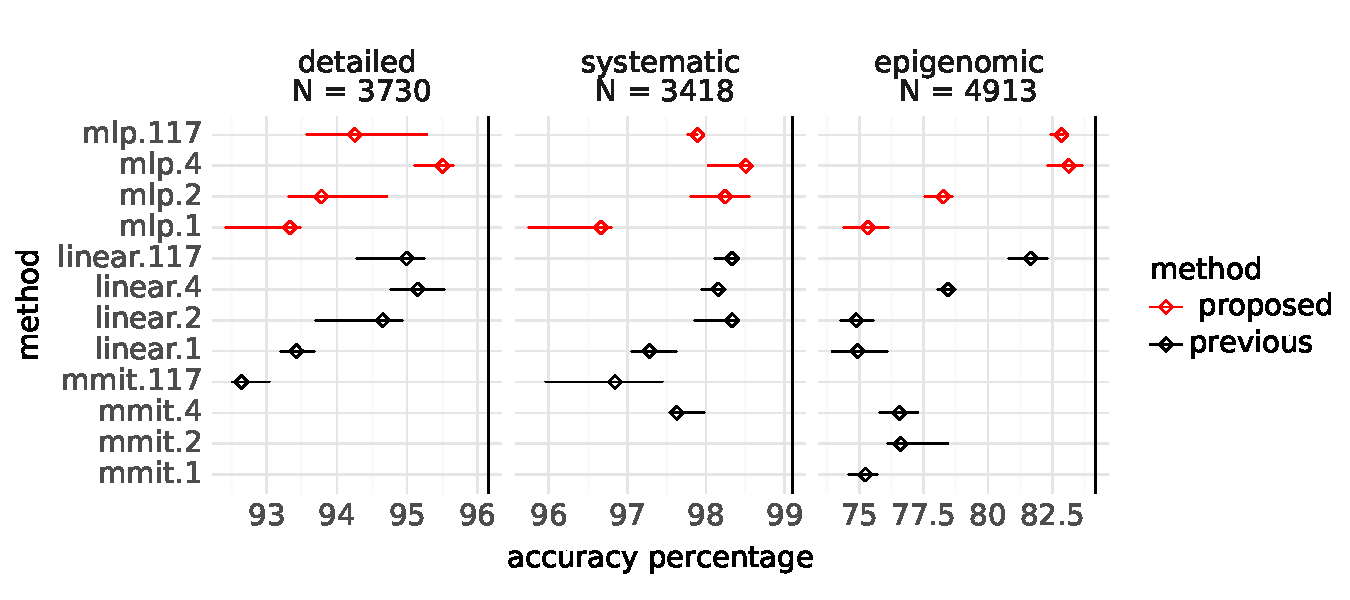
\includegraphics[width=0.9\textwidth]{figs/fig.acc_compare}
\caption{Median test accuracy and interquartile across 6 folds for each method}
\label{fig:acc_comp}
\end{figure}

\begin{table}[!t]
\centering
\begin{tabular}{llllll}
\hline
\textbf{Dataset} & \textbf{Sequences} & \textbf{Pos. Labels} & \textbf{Neg. Labels} & \textbf{Source} \\ \hline
{Detailed}       & 3730                    & 964                  & 3396                 & \href{https://github.com/tdhock/neuroblastoma-data/tree/master/data/detailed}{GitHub} \\ \hline
{Systematic}     & 3418                    & 573                  & 2846                 & \href{https://github.com/tdhock/neuroblastoma-data/tree/master/data/systematic}{GitHub}  \\ \hline
{Epigenomic}     & 4913                    & 2185                 & 8195                 & \href{https://archive.ics.uci.edu/ml/machine-learning-databases/00439/peak-detection-data.tar.xz}{UCI Repo} \\ \hline
\end{tabular}
\label{tab:datasets}
\caption{Datasets used in the study}
\end{table}

\subsubsection{Experiments and Results}

\paragraph{Features} Four sets of features are considered to evaluate their quality:
\begin{itemize} 
\item \textbf{1 feature}: Sequence length, as used in \cite{hocking:20} and \cite{bic}. 
\item \textbf{2 features}: Sequence length and variance, following \cite{rigaill:13}. 
\item \textbf{4 features}: Sequence length, variance, value range, sum of absolute differences. 
\item \textbf{All features}: According to \cite{rigaill:13} and \cite{mmit}, up to 365 features are generated, with only those without of missing data, infinite values, or zero variance retained.
\end{itemize}

\paragraph{Models Configuration}
All models employed 5-fold cross-validation to select the optimal hyperparameters.
\begin{itemize}
    \item \textbf{Linear}: L1 regularization is applied only to the large feature vector, with cross-validation used to determine the optimal L1 parameter value, starting at 0.001 and increasing by 1.2 until no features remain.

    \item \textbf{MMIT}:
The hyperparameters considered include a list for \texttt{max\_depth} values (0, 1, 5, 10, 20, Inf), \texttt{margin} (0, 1, 2) ($\epsilon$ from equation \ref{eq:loss_func}), \texttt{loss\_type} (\texttt{hinge}, \texttt{square} -- equivalent to $p=1$ or $p=2$ in Equation \ref{eq:loss_func}) and \texttt{min\_sample} (0, 1, 2, 4, 8, 16, 20).

    \item \textbf{AFT in XGBoost}: 
The hyperparameters considered include a list of \texttt{learning\_rate} values (0.001, 0.01, 0.1, 1.0), \texttt{max\_depth} (2, 3, 4, 5, 6, 7, 8, 9 10), \texttt{min\_child\_weight} (0.001, 0.1, 1.0, 10.0, 100.0), \texttt{reg\_alpha} (0.001, 0.01, 0.1, 1.0, 10.0, 100.0), \texttt{reg\_lambda} (0.001, 0.01, 0.1, 1.0, 10.0, 100.0), \texttt{aft\_loss\_distribution\_scale} (0.5, 0.8, 1.1, 1.4, 1.7, 2.0).
This setup is identical to that described in \citep{barnwal2022survival}.

    \item \textbf{MLP}: The hyperparameters considered include a list of \texttt{n\_hidden\_layer} (1, 2, 3, 4) and \texttt{hidden\_layer\_size} (2, 4, 8, 16, 32, 64, 128, 256, 512). We used the early stopping technique using a \texttt{patience} parameter, stopping training if the loss does not decrease after the specified patience iterations; in our study, we set the maximum iterations to 12,000 and the patience to 20. The model is trained using the Adam optimizer (with default PyTorch hyperparameters) to minimize the Squared Hinge Loss (as defined in Function \ref{eq:loss_func} with $p=2$ and $\epsilon=1$).
\end{itemize}

\paragraph{Results} This study uses 3 large datasets, as detailed in Table \ref{tab:datasets}.
Each dataset is split into 6 similar size folds.
In each iteration, 1 fold is designated as the test set, and the remaining 5 folds form the train set, with the process yield 6 test accuracy rates (Figure \ref{fig:acc_comp}) and F1 scores (Figure \ref{fig:F1_comp}) for each method.

\begin{figure}[!t]
\centering
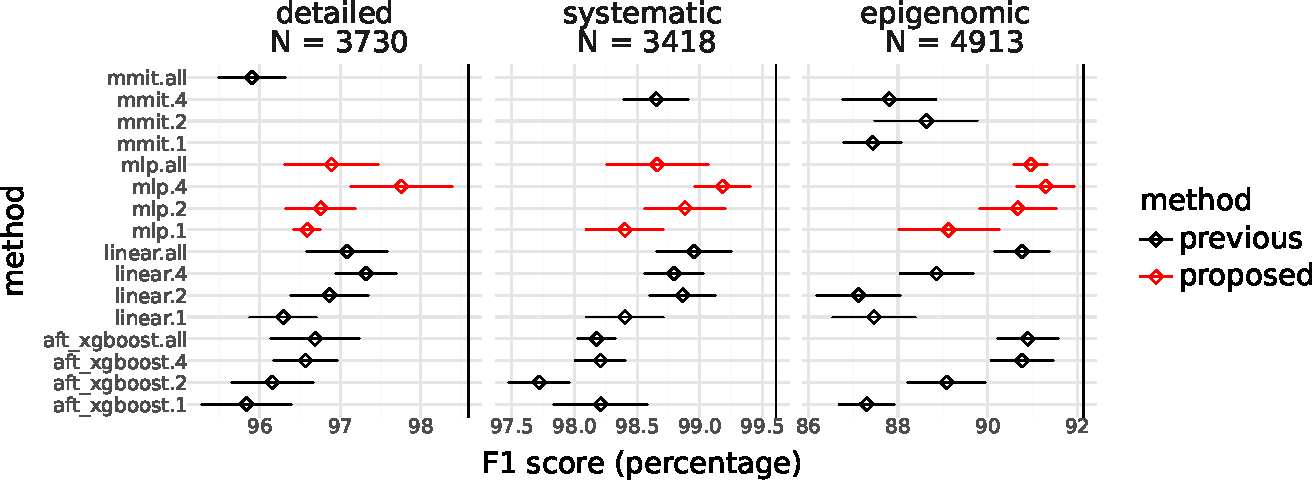
\includegraphics[width=0.9\textwidth]{figs/fig.F1_compare}
\caption{Median test F1 score and interquartile across 6 folds for each method.}
\label{fig:F1_comp}
\end{figure}

\subsubsection{Discussion and Conclusion}

\paragraph{Performance Analysis and Overall Comparison}

Figures \ref{fig:acc_comp} and \ref{fig:F1_comp} demonstrate that the proposed model, when trained with the selected four-feature configuration, consistently achieves comparable or slightly superior performance relative to previously published linear and tree-based approaches across all evaluated datasets. Although the observed improvements in mean accuracy and F1 score are modest, they are stable across cross-validation folds, indicating that the gains are systematic rather than incidental. 

In particular, increasing the number of features from one to two and then to four generally leads to improved predictive performance for all model families considered. This trend suggests that the selected features provide complementary information that enhances the model’s ability to correctly identify changepoint intervals. However, the inclusion of all available features does not necessarily yield further improvement. In several cases, performance stagnates or slightly deteriorates when all features are used, indicating the presence of redundant or weakly informative variables. This highlights the importance of careful feature selection, especially for flexible models such as MLPs.

\paragraph{Comparison Between Model Families}

A notable observation is that tree-based models do not consistently outperform linear models when trained on the same feature sets. This phenomenon aligns with findings reported in \citep{mmit} for the Systematic dataset and in \citep{barnwal2022survival} for subsets of the Epigenomic dataset. The primary reason appears to be the predominantly linear relationship between the extracted features and the target intervals, as illustrated in Figure \ref{fig:features_targets}. When the underlying structure of the data is largely linear, more complex nonlinear learners such as tree ensembles do not offer a significant advantage.

The proposed model, formulated as a piecewise linear MLP, is conceptually positioned between purely linear models and highly nonlinear deep architectures. As expected, for identical feature configurations, it generally outperforms the standard linear model. The improvement can be attributed to its ability to capture mild nonlinearities while preserving much of the interpretability and stability of linear approaches. Importantly, strong performance is achieved with a relatively simple architecture—typically a single hidden layer containing 4 or 8 neurons—demonstrating that excessive architectural complexity is unnecessary for these datasets.

\begin{figure}[!t]
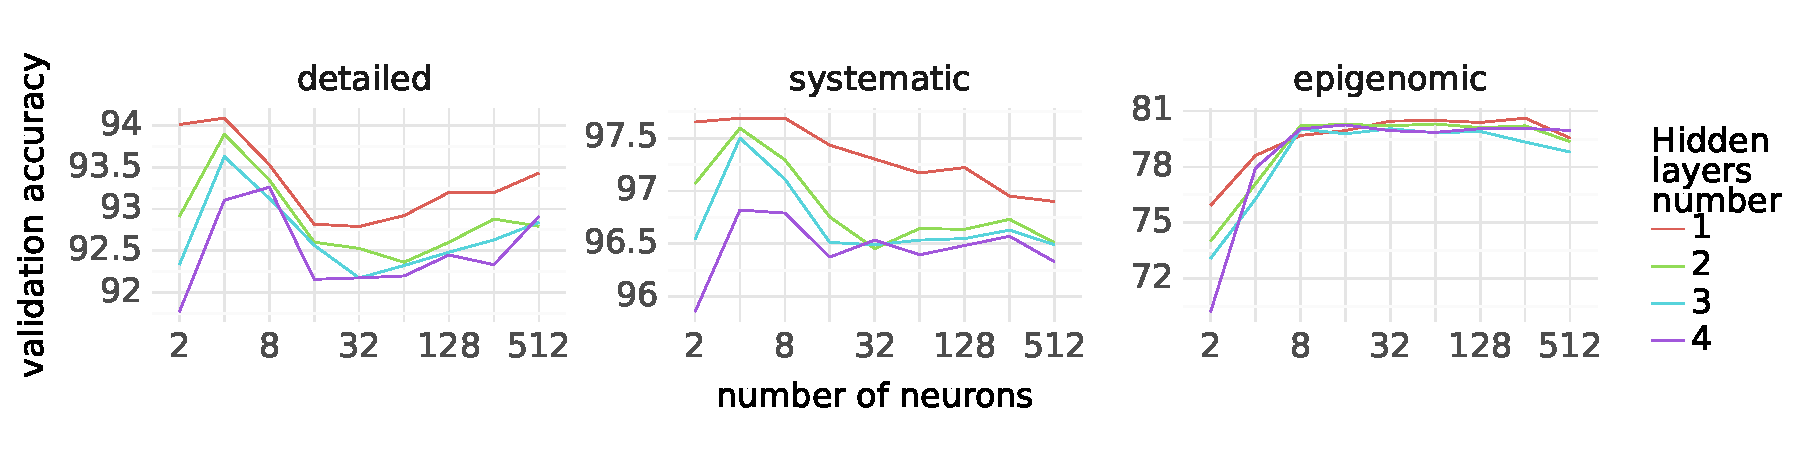
\includegraphics[width=0.99\textwidth]{figs/fig.mlp}
\caption{Average validation accuracies for different MLP configurations}
\label{fig:mlp}
\end{figure}

\paragraph{Consistency and Stability of the Proposed Model}

While the proposed model achieves strong mean performance, Figures \ref{fig:acc_comp} and \ref{fig:F1_comp} also indicate that MLPs tend to exhibit wider confidence intervals compared to linear and tree-based models. This variability likely stems from the higher sensitivity of neural networks to initialization, optimization dynamics, and hyperparameter configurations. Despite this increased variance, the overall performance remains competitive and robust across folds. The results suggest that moderate architectural simplicity contributes to improved stability without sacrificing predictive power.

\paragraph{Factors Affecting Performance}
\begin{itemize}
    \item \textit{Feature Design.} The experiments confirm that feature quality plays a more critical role than model complexity. The relationship between sequence length and the target interval of $\lambda$, as shown in Figure \ref{fig:features_targets}, is not clearly separable, which may explain why models trained solely on this feature underperform relative to those incorporating additional statistical descriptors such as variance or range. The fact that nonlinear models do not benefit from the inclusion of all features further underscores that feature relevance, rather than feature quantity, determines performance gains.
    \item \textit{MLP Configuration.} Determining an effective MLP configuration required systematic experimentation. We evaluated 36 distinct configurations for each train–test pair by varying the number of hidden layers (1–4) and the number of neurons per layer (2 to 512, in powers of two). This grid search was computationally demanding. Nevertheless, results indicate that shallow architectures with limited width are sufficient. Given the largely linear structure of the problem, deeper or wider networks did not provide consistent improvements, reinforcing the principle that model capacity should match data complexity.
\end{itemize}



\paragraph{Limitations}

Several limitations should be acknowledged. First, feature extraction was performed manually, and only a limited subset of possible statistical descriptors was considered. The space of potential features derivable from sequences is effectively unbounded; measures such as skewness, kurtosis, entropy, or counts of repeated values were not included. Consequently, potentially informative predictors may have been overlooked.

Second, unlike L1-regularized linear models or tree-based algorithms, MLPs lack an inherent feature selection mechanism. This limitation reduces flexibility when handling larger feature spaces and increases the risk of incorporating redundant variables. As a result, careful preprocessing remains essential for neural network models in this setting.

Third, identifying optimal MLP hyperparameters is time-consuming and computationally intensive. Although an extensive search was conducted, configurations with heterogeneous neuron counts across layers were not explored, leaving open the possibility that alternative architectures could yield marginal improvements.

\paragraph{Conclusion and Future Directions}

Overall, the proposed piecewise linear MLP model achieves comparable or slightly improved accuracy and F1 scores in changepoint detection relative to traditional linear and tree-based models. The results emphasize that thoughtful feature selection is more influential than architectural complexity. While the model benefits from moderate nonlinear flexibility, its performance does not justify highly complex network designs for the datasets studied.

Future research may focus on automating feature learning rather than relying on manual extraction. In particular, sequence-oriented neural architectures such as Recurrent Neural Networks (RNNs) \citep{rnn}, Gated Recurrent Units (GRUs) \citep{gru}, and Long Short-Term Memory (LSTM) networks \citep{lstm} could be investigated for directly learning informative representations from raw sequences. Such approaches may alleviate the need for handcrafted features and potentially enhance generalization to other sequence domains.

\paragraph{Reproducible Research Material}

To promote transparency and facilitate replication, all source code and experimental materials are publicly available at: \href{https://github.com/lamtung16/ML_ChangepointDetection}{github}. Providing open access to the implementation ensures that results can be independently verified and extended by future researchers.


\newpage

\subsection{Optimal Partitioning Penalty Learning: Recurrent}

Changepoint detection (other words, partitioning or segmentation) is important for identifying abrupt changes in data in various domains, including finance \citep{app:finance}, healthcare \citep{cancer}, network security \citep{app:network}, and environmental science \citep{app:climate}. This importance has driven the development of numerous methods over the past decades.

\paragraph{Changepoint Detection Methods.}
Changepoint detection methods can be divided into two categories: Deep Learning (DL) and Dynamic Programming (DP).
 
DL-based methods, which inspired from a statistical method Cumulative Sum (CUSUM) \citep{review:cusum, review:james1987tests}, including recent works \citep{review:li24automatic, review:ermshaus2023clasp} employ multilayer perceptrons (MLP) or k-nearest neighbors (KNN) as classification sliding windows to identify changepoints. 
However, these methods rely on local neighbors rather than the entire sequence and are overly complex for univariate data.

In contrast, DP is well-suited for this context.
These algorithms rely on a single hyperparameter to limit the changepoints number, which can be either: (a) a fixed changepoints number or (b) a penalty parameter to penalize the changepoint presence.
Fixed changepoints number allow DP algorithms \citep{review:binseg, review:bai2003computation, review:pelt, rigaill2015pruned} to locate them, but the changepoints number is rarely predetermined.
More commonly used, penalty-based DP algorithms, such as Optimal Partitioning (OPART) \citep{review:opart} and its variants—Pruned Exact Linear Time (PELT) \citep{review:pelt}, Functional Pruning Optimal Partitioning (FPOP) \citep{review:fpop}, and Labeled Optimal Partitioning (LOPART) \citep{review:lopart}—are widely regarded as the most effective.
PELT and FPOP prune candidate changepoints efficiently, producing identical partitions as OPART, while LOPART extends OPART by incorporating predefined labels (the expected number of changepoints within specific location ranges) or defaulting to OPART when labels are absent.
The following is the OPART optimization problem:

\paragraph{OPART Problem.} Given a sequence $\mathbf{d} \in \mathbb{R}^N$ and penalty parameter $\lambda \geq 0$,
find the vector $\mathbf{m} \in \mathbb{R}^N$ that minimizes the following cost function:
\begin{equation*} \label{eq:opart_loss}
C(\textbf{d}, \textbf{m}) + \lambda M
\end{equation*}
\noindent Here, $C(\textbf{d}, \textbf{m})$ represents the error between the sequence $\textbf{d}$ and the vector $\textbf{m}$ and $M$ is the number of changes in $\textbf{m}$.
The formula of $C(\textbf{d}, \textbf{m})$ and $M$ depends on the type of change.
If the type of change is mean, then $C(\textbf{d}, \textbf{m}) = \sum_{i=1}^{N}(m_i-d_i)^2$ and $M=\sum_{i=1}^{N-1} I[m_i \neq m_{i+1}]$, where $I[m_i \neq m_{i+1}]$ equals 1 if a changepoint occurs ($m_i \neq m_{i+1}$) and 0 otherwise.
\newline

In OPART algorithms, the penalty plays a key role.
A higher penalty imposes a stronger penalty on changepoint presence, leading to fewer changepoints, see Figure \ref{fig:lambda}.
This study aims to predict that penalty to improve the changepoint detection accuracy. 
From here on, that conceptual penalty will be referred to as $\lambda$.

\paragraph{Existing $\lambda$ prediction models.}
Various models exist for predicting $\lambda$, including unsupervised \citep{bic, aic, lavielle05} and supervised such as linear \citep{rigaill:13} and tree(s) \citep{mmit, barnwal2022survival}.
But all of these models rely on a set of manually extracted sequence features, yet the number of possible features is infinite, this process can result in the inclusion of many irrelevant features, and the potential omission of useful ones.

\paragraph{(iv) (v) Contribution.} This study proposes a novel method utilizing a recurrent network to automatically extract relevant features from sequences, which are then used to predict $\lambda$.
Experiments on benchmark datasets show that the proposed method achieves higher partitioning accuracy than existing ones in most cases.

\paragraph{Reproducibility.} To ensure transparency, the code used for this study is accessible at: \url{https://github.com/lamtung16/ML_Changepoint_Detection_epigenomic_rnn}.


\subsubsection{Contribution}
\paragraph{Feature Extraction via Recurrent Networks.} In a Recurrent Network with input size \(k \geq 1\) and hidden size \(m \geq 1\), processing a sequence \(\mathbf{d} = [d_1, d_2, \dots, d_N] \in \mathbb{R}^N\), the hidden state at time \(t\), called $h_t$, is updated as:
\[
h_t = f(d_{[t:t+k-1]}; h_{t-1}) \in \mathbb{R}^m
\]
where $d_{[t:t+k-1]} = [d_{t}, d_{t+1}, ..., d_{t+k-1}] \in \mathbb{R}^k$.
Time stamp \(t\) ranges from $k$ to \(N\).
The initial hidden state \(h_{k-1}\) can be assigned manually.
The final hidden state \(h_N \in \mathbb{R}^m\) captures information from the entire sequence.
Thus, we use \(h_N\) as the \(m\) extracted features from the raw sequence. 

\paragraph{Predicting $\lambda$ from extracted features.}
The prediction is formed by the linear combination of $m$ extracted features:
$$\log \lambda = h_N \cdot \beta + \beta_0$$
where \(\beta \in \mathbb{R}^m\) and \(\beta_0 \in \mathbb{R}\) are the parameters to be learned.


\begin{figure}[!t]
\vskip 0.2in
\begin{center}
\centerline{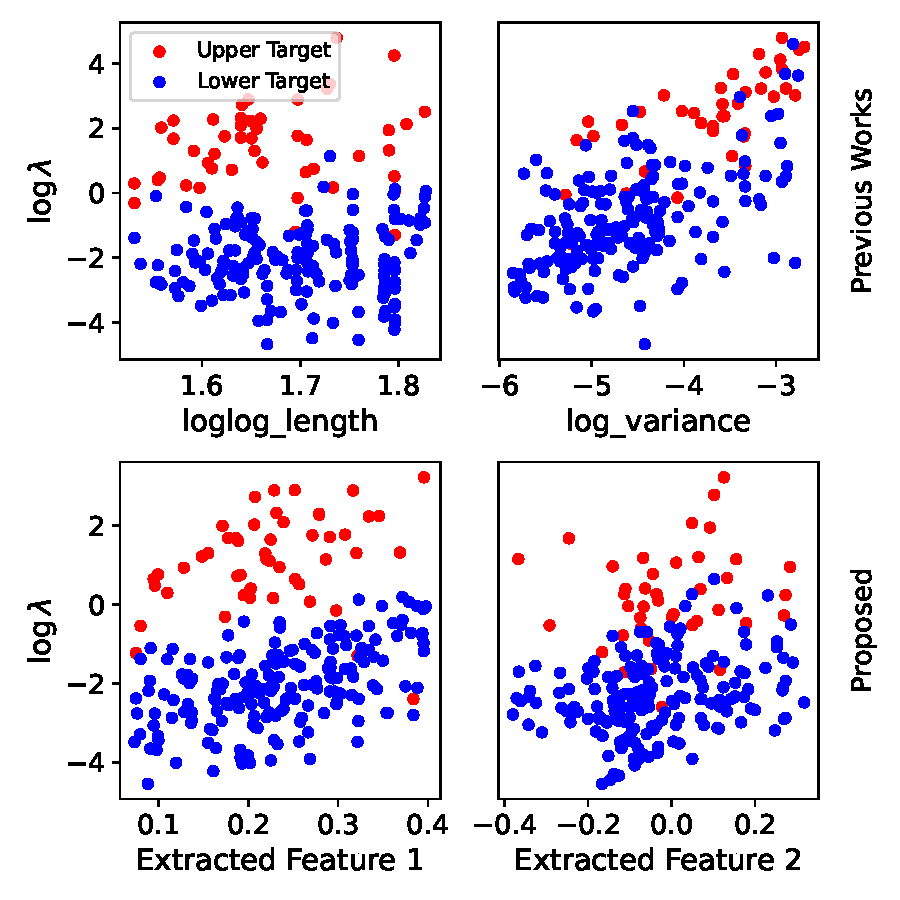
\includegraphics[width=0.7\textwidth]{figs/figure.5_extracted_features.pdf}}
\caption{Example: features vs. targets from the dataset detailed}
\label{fig:extracted_features}
\end{center}
\vskip -0.2in
\end{figure}


\paragraph{Automatic extracted features vs. Manual extracted features.} The novel method generates useful features without the need for a large number, unlike previous models.
Figure \ref{fig:extracted_features} provides an example by comparing the ability to predict $\lambda$ using length (or variance) - as these manual extracted features are considered key for $\lambda$ prediction in unsupervised methods - versus automatic extracted features from recurrent networks.
It demonstrates that the automatic extracted features probably provide a more accurate prediction of $\lambda$ than either length or variance.

\paragraph{Feature Approximation Ability of Recurrent Networks.}
Recurrent networks have the ability to approximate statistical sequence features. For example, if the core network is defined as \( h_t = h_{t-1} + 1 \) when \( h_0 = 0 \) and the input size $k = 1$, then \( h_N = N \), which represents the sequence length, a feature used in BIC. 
The core component of these models is a deep neural network. 
For instance, the Vanilla Recurrent Network \citep{rnn} core is a MLP, which, according to the universal approximation theorem \citep{mlp}, can approximate any continuous function, regardless of its complexity, provided there are enough neurons in the hidden layer. 
This is why, although these models may not directly produce exact statistical sequence features, their architecture enables them to approximate these features with a high degree of accuracy.

\paragraph{Recurrent networks to be implemented.} This study explores three recurrent networks: Vanilla Recurrent Network (RNN), Long Short-Term Memory (LSTM) \citep{lstm}, Gated Recurrent Unit (GRU) \citep{gru}.
RNNs struggle with long-term dependencies due to the vanishing gradient problem. 
LSTMs address this by introducing memory cells and gating mechanisms that help retain information over longer sequences. 
GRUs, a simplified version of LSTMs, combine the forget and input gates into a single update gate, offering a more efficient alternative while still capturing long-term dependencies.

\begin{figure}[tb]
\vskip 0.2in
\begin{center}
\centerline{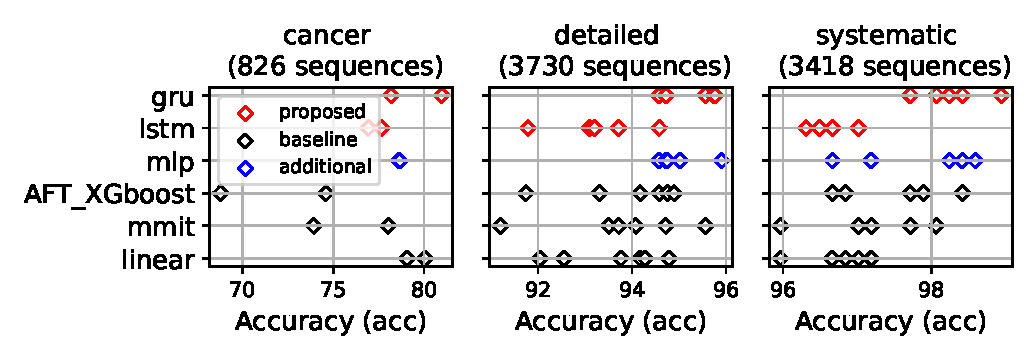
\includegraphics[width=0.7\textwidth]{figs/figure.4_acc_no_pooling.pdf}}
\caption{The accuracies for each fold are presented for datasets without any pooling}
\label{fig:acc_no_pooling}
\end{center}
\vskip -0.2in
\end{figure}

\subsubsection{Experiments and Results}
The comprehensive accuracy results of all 8 methods for each of 20 datasets are provided in the Appendix, as the table is too large to be included in the main paper.
Figure \ref{fig:acc_no_pooling} presents the accuracy rates for three datasets using the original, unpooled sequences.
Each dataset is evaluated using seven different methods, producing multiple accuracy values depending on the number of folds used for that dataset.

\subsubsection{Discussion and Conclusion}
\paragraph{Summary of Contributions.}
Technically, these proposed models still perform two steps: (1) Feature extraction and (2) Predicting $\lambda$ based on the extracted features.
However, instead of performing these steps separately, it combines them into a single operation, enhancing its robustness compared to previous models.
Automatic extracting features helps generate highly useful ones without requiring many features, as shown in Figure \ref{fig:extracted_features}.
This study focuses exclusively on genomic datasets, where prior knowledge of relevant features enables effective manual feature extraction. 
However, the proposed models stand out because it does not require expert knowledge to perform. Its automatic feature extraction mechanism makes it versatile and applicable to any type of sequence dataset.

\paragraph{Comparison to Previous Models.}
Recurrent networks, in general, outperform previous models across datasets, see Figure \ref{fig:acc_no_pooling}.
For small datasets (with fewer than 100 instances), the accuracy of the proposed models is comparable (neither better nor worse) to that of existing models. 
On the other hand, when dealing with larger datasets, recurrent networks noticeably outperform previous models and show a slight edge over MLPs.

\paragraph{Comparison between Recurrent Networks.}
When comparing RNN, LSTM, and GRU, as expected, RNN performs the worst due to its difficulty with long-term memory. 
In most cases, GRU outperforms the others.

\begin{figure}[!t]
\vskip 0.2in
\begin{center}
\centerline{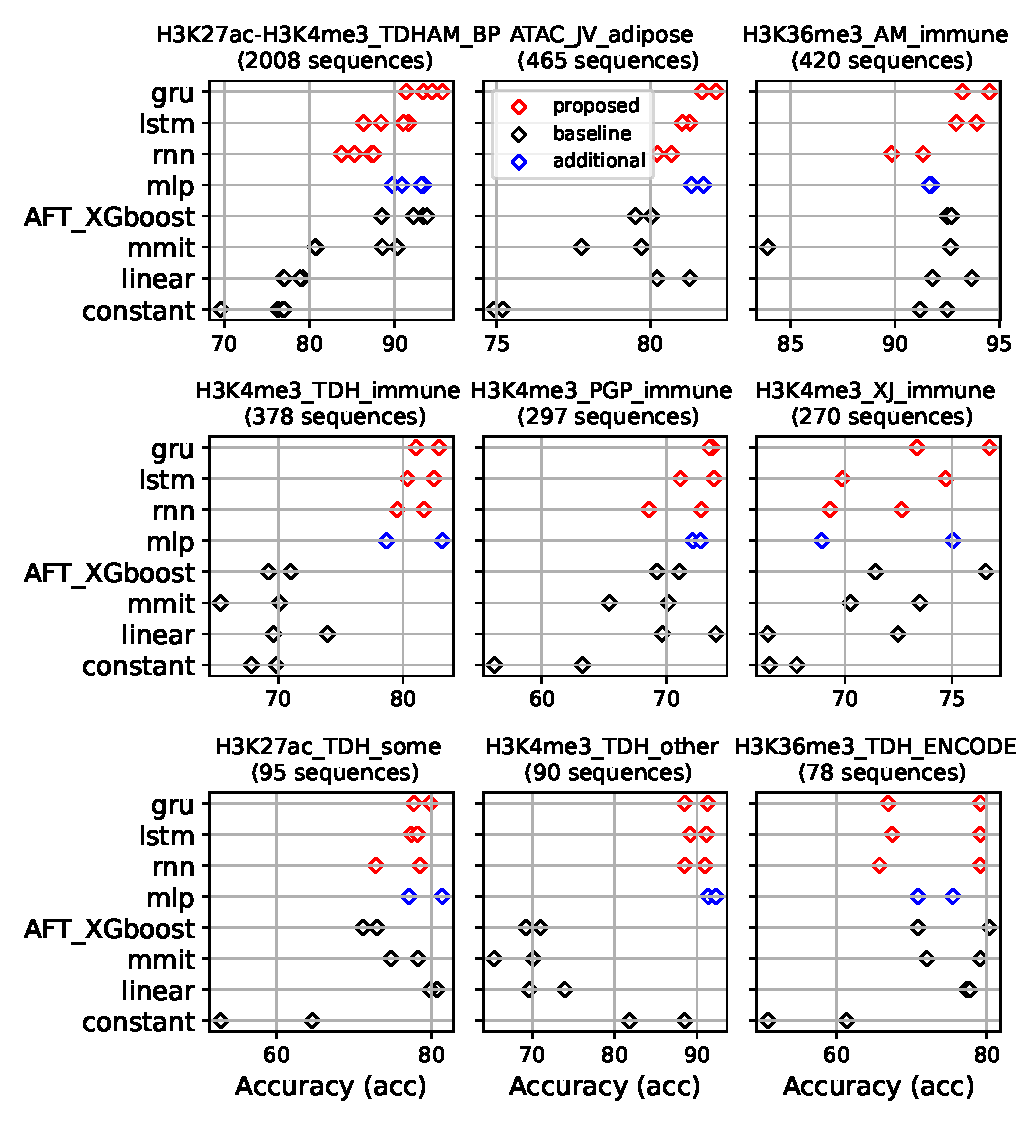
\includegraphics[width=0.7\textwidth]{figs/figure.4_acc_chipseq.pdf}}
\caption{The fold accuracies on some ChIP-seq datasets}
\label{fig:acc_chipseq}
\end{center}
\vskip -0.2in
\end{figure}

\paragraph{Discussion on the Number of Automatically Extracted Features.}  
The number of automatic extracted features needs to be sufficiently large. 
It is observed that when 8 or 16 features are extracted, the validation loss value is slightly smaller compared to when only 2 or 4 features are extracted.

\paragraph{Impact of pooling preprocessing.}
Shortening the sequence for training is effective. As the window size increases, more information is lost. 
However, when the window size is small, such as 100, the performance of the recurrent models is worse compared to larger window sizes like 1000 or 2000. This could be because the pooled sequence with a window size of 100 is still too long for the recurrent models to handle effectively. 
The pooling process is beneficial in two ways: it can improve the accuracy of recurrent networks and also reduce training time.
We employed two pooling functions, mean and median, to represent a single value for each non-overlapping window. 
It is evident that using the mean value as the representation consistently yields smaller loss.

\paragraph{Study Limitations.}
Although the Recurrent Network architecture is straightforward, as its core essentially a deep neural network, training these models can be time-consuming due to the inherently sequential nature of the process.
For some train/test pairs, even after applying pooling to reduce the sequence length, training a model with a maximum of 2 layers, each containing no more than 16 neurons, and a maximum of 1000 iterations, took over approximately 10 days, despite utilizing the powerful NVIDIA A100 GPU.
These models also require significant memory to store the hidden states at each time step. 
To avoid out-of-memory (OOM) errors, it is crucial to allocate sufficient memory, especially for long sequences.

\begin{figure}[!t]
\vskip 0.2in
\begin{center}
\centerline{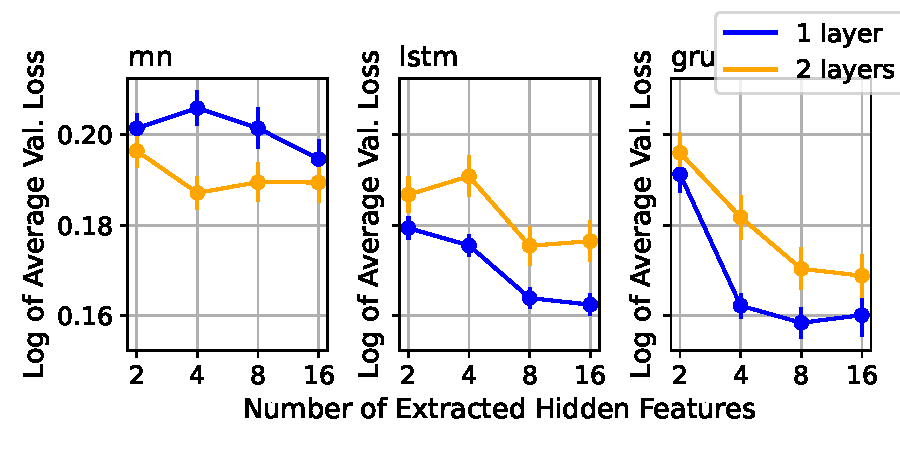
\includegraphics[width=0.7\textwidth]{figs/figure.5_n_extracted_features.pdf}}
\caption{Log of the loss validation across different numbers of extracted hidden layers}
\label{fig:n_feature}
\end{center}
\vskip -0.2in
\end{figure}

\paragraph{Practical Considerations in Real-World Applications.}
There is a trade-off between training time and accuracy. 
The proposed models have higher accuracy in most of the 20 datasets, but they are significantly more time-consuming to train, especially for longer sequences. 
In contrast, manually extracted features models do not face this issue.
Therefore, in real-world scenarios where datasets contain only a few sequences but each sequence is long, and training time is a priority, manually extracted features models may be the better choice for two reasons: first, their training time is significantly faster; and second, these models' accuracy is comparable to the proposed models.
However, if the user’s priority is accuracy and the hardware requirements are met, the proposed models are a better choice.
Although the training process is time-consuming, it only needs to be done once; afterwards, the trained models can be applied to unseen sequences, as their feed-forward process is sufficiently fast.



\paragraph{Future Directions.}
For these particular datasets, it is assumed that $\lambda$ exhibits an increasingly monotonic behavior with respect to both sequence length and variance, which are employed in unsupervised methods. 
One approach is to leverage monotonic network architectures, such as min-max networks \citep{monotonic}, or more advanced architectures like Lattice Networks \citep{lattice}, with modifications to the loss function for each linear region.

We can consider CNNs \citep{cnn} because they are capable of handling sequences of varying lengths and generating a single output by utilizing convolution layers to extract features across the sequence. 
Global pooling layers (e.g., Global Max or Average Pooling) aggregate these features into a fixed-size representation. This vector is then passed through a MLP to produce the final output.

To build upon the initial concept of utilizing recurrent networks in this study, various types of models could be explored in the future:
\begin{itemize}
    \item Using a more complex model: This study predicts $\lambda$ by using a linear combination of the extracted features. Alternatively, we could consider using a more complex model such as MLP that processes the extracted features instead of relying on a linear combination.
    \item Attention mechanisms \citep{attention} dynamically focus on relevant input parts, assigning importance weights to subsequences. Unlike sequential RNNs, they effectively capture long-range dependencies and handle varying input lengths, making them ideal for this task.
    \item Bidirectional Recurrent Networks \citep{bidirectional}: The models implemented in this study are unidirectional, leading to challenges with long-term memory, since the later parts of the sequence tend to be more important than the earlier ones. Using a bidirectional recurrent network architecture can aim to address this limitation, enabling the model to better capture information from the sequence.
\end{itemize}



Conducting even a preliminary experiment would require substantial computing resources, since bidirectional networks and attention mechanisms are more computationally expensive than the proposed one. For this reason, we chose not to include such experiments as part of this work.

\newpage
\subsection{Interval Regression: Review}
In addition to existing state-of-the-art models, this study proposes several alternative models, including common machine learning architectures such as KNN, Neural Networks, and Random Forests, to provide a more comprehensive comparison.

\subsubsection{Contribution}
\paragraph{K-Nearest Neighbors (KNN)} KNN is a classical model for Standard Regression, which motivates its consideration in the Interval Regression setting.
The Interval Regression procedure follows the same steps as the standard KNN regression model \citep{knn}, with the key difference being how the regression value is determined from the \( k \) nearest neighbors.
We propose utilizing the MMIT regression function. 
Specifically, we treat the set of \( k \) nearest neighbors as a single leaf in a MMIT, where the regression value is a constant that minimizes the mean Hinge Error \eqref{eq:lossfunction} between this constant and the \( k \) target intervals.
The prediction $\hat{y}$ based on the target intervals of the \( k \) nearest neighbors, denoted as \( \{(y_l^i, y_u^i)\}_{i=1}^k \), is formulated as:
\[
    \hat{y} = \argmin_c \frac{1}{k} \sum_{i=1}^{k} l\big(c, (y_l^i, y_u^i)\big), \quad c \in \{y_l^i, y_u^i, \frac{y_l^i + y_u^i}{2}|y_l^i > -\infty, y_u^i < \infty\}_{i = 1}^k
\]

\paragraph{Multilayer Perceptron (MLP)} Since MLP is a commonly used neural network in Standard Regression models \citep{uni_approximator}, its application in Interval Regression is worth considering.
The training process of this model is the same as in the linear model \textit{Max Margin Interval Regression}.

\paragraph{Maximum Margin Interval Forest (MMIF)} The idea of using ensembles of MMITs was mentioned in Chapter 6 (Discussion and Conclusions) of \citep{mmit}. 
Since MMIT is a tree for the Interval Regression setting, its extension to construct a Random Forest for Interval Regression is straightforward.  
The operation of MMIF follows the same principles as the standard Random Forest regressor \citep{rf}, with the key distinction being that MMITs are used instead of conventional decision trees.

\begin{figure}[!t]
\vskip 0.2in
\begin{center}
\centerline{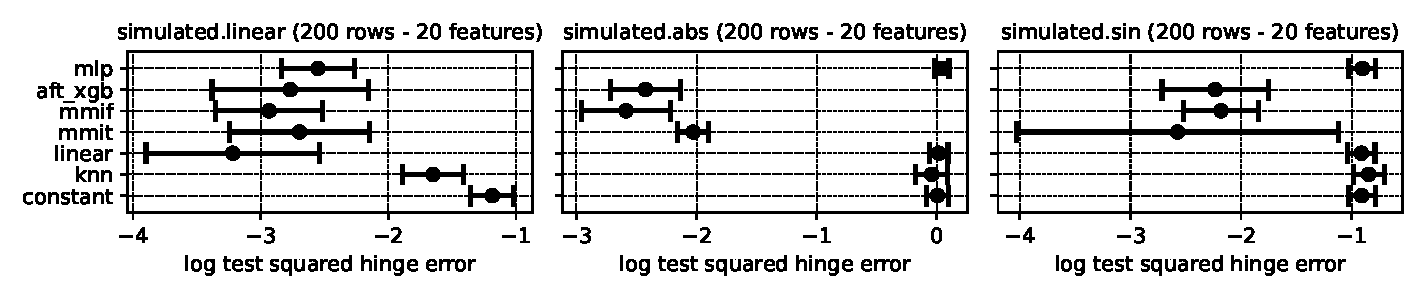
\includegraphics[width=1\textwidth]{figs/fig.results_simulated.pdf}}
\caption{The mean and standard deviation of the test squared hinge errors in simulated datasets}
\label{fig:err_simulated}
\end{center}
\vskip -0.2in
\end{figure}

\subsubsection{Experiments and Results}
For each of the 39 datasets, 7 models were implemented, with each model producing 5 hinge error values (corresponding to 5 train/test pairs).

\subsubsection{Discussions and Conclusions} \label{sec:discussion}
\paragraph{Dataset Variations.}
To ensure a comprehensive comparison, the quality of the datasets is important.
The datasets employed have a variety of characteristics, including high- and low-dimensional data, real-world and synthetic sources, linear and nonlinear patterns, as well as low- and high-noise conditions. 


\paragraph{Comprehensive Comparison.}
The performance and consistency rankings are in Table \ref{tab:comparison}, 1st means the best and 7th means the worst. 
About the performance, it's clear that MMIF outperforms other models in most cases. 
Linear, MMIT and MLP are comparable, while Constant, kNN, and the AFT model in XGBoost show the poorest performance.
About the consistency, MMIF stands out as the most consistent. 
This is expected, as MMIF being an ensemble model, relies on a group of MMITs to make the final prediction, which helps improve its stability.
Again, Constant, kNN, and the AFT model in XGBoost show the lowest consistency.

\paragraph{No single model is optimal for all scenarios.}  
As shown in Table \ref{tab:comparison}, there is no universally optimal model for every scenario.
However, if complexity is not a primary concern, and the goal is to select the model with the best overall performance and consistency, MMIF is likely the first choice.  
Alternatively, if model complexity and training time are critical factors, MMIT is preferable, as it's less complex than MMIF, require significantly fewer training resources, and still maintain reliable performance.

\paragraph{MMIT vs MMIF.} 
This is a comparison worth considering.
MMIF was proposed with the expectation that an ensemble of MMITs would outperform a single MMIT, and the results confirm this hypothesis. 
Specifically, across 39 datasets, MMIF outperformed MMIT in 28 of them. 
This makes sense: MMIF, being an ensemble of MMITs, is able to reduce overfitting by not relying on a single MMIT.

\paragraph{Discussion on the AFT Model in XGBoost.}
The AFT model in XGBoost is the complex models in this study, but its performance and consistency do not justify the complexity. 
% It has a limitation in that it can only handle non-negative target intervals. 
To make the model applicable to a general Interval Regression setting, the target intervals must be transformed using exponential function. 
So the model becomes highly sensitive when the dataset contains many left-censored target intervals. 
When predictions are made on the exponential scale, if the predicted value is close to zero, the mapping back to the original scale can result in large negative values.
% as seen in some test cases where predictions like $-10^6$ were made.
\[
(-\infty, y_u) \overset{\text{exp}}{\longrightarrow} (0, \exp y_u) \overset{\text{predict}}{\longrightarrow} y_p \approx 0 \overset{\text{log}}{\longrightarrow} \hat{y} \approx -\infty \overset{\text{evaluate}}{\longrightarrow} \text{Big test error}
\]
The Figure 2.b in \citep{aft_xgboost} indicates that the AFT model in XGBoost performs among the worst across their six simulated datasets when compared to the Linear and MMIT. 

A potential direction for future work is to transform left-censored intervals into interval-censored intervals by replacing all lower bounds of \(-\infty\) with a finite value. This adjustment aims to reduce the model's sensitivity to left-censored intervals and mitigate the tendency to produce excessively large negative predictions.

\begin{table}[t!]
\centering
\begin{tabular}{l|rrrrrrr|rrrrrrr}
\toprule
 & \multicolumn{7}{c|}{Performance} & \multicolumn{7}{c}{Consistency} \\
\midrule
 & 1st & 2nd & 3rd & 4th & 5th & 6th & 7th & 1st & 2nd & 3rd & 4th & 5th & 6th & 7th \\
\midrule
constant & 2 & 2 & 3 & 1 & 4 & 7 & 20 & 4 & 0 & 2 & 3 & 3 & 8 & 19 \\
knn & 4 & 4 & 2 & 6 & 6 & 16 & 1 & 4 & 3 & 3 & 7 & 7 & 12 & 3 \\
linear & 3 & 11 & 6 & 8 & 5 & 5 & 1 & 7 & 7 & 8 & 7 & 7 & 3 & 0 \\
mmit & 2 & 10 & 9 & 3 & 9 & 4 & 2 & 2 & 13 & 4 & 8 & 8 & 2 & 2 \\
mmif & 15 & 5 & 8 & 7 & 4 & 0 & 0 & 12 & 9 & 9 & 4 & 3 & 2 & 0 \\
aft\_xgb & 4 & 4 & 3 & 4 & 7 & 5 & 12 & 4 & 1 & 7 & 2 & 3 & 10 & 12 \\
mlp & 9 & 3 & 8 & 10 & 4 & 2 & 3 & 6 & 6 & 6 & 8 & 8 & 2 & 3 \\
\bottomrule
\end{tabular}
\caption{The comparison of the performance and consistency of 7 interval regression models}
\label{tab:comparison}
\end{table}

\newpage
\thispagestyle{empty}
\bibliographystyle{abbrvnat}
\bibliography{references}

\end{document}